%=========================================================================
% (c) Michal Bidlo, Bohuslav Křena, 2008

\chapter{Úvod}
\phantomsection
Rozpoznávání řeči je oblast, která je už po dlouhou dobu aktuální a neustále se posouvá kupředu. Je velice užitečné pro usnadnění mnoha činností, ať už se jedná o~převod přednášek do textové podoby nebo osobního asistenta v~mobilních zařízeních. Vzhledem k~nárustu výpočetní kapacity v~zařízeních, jako jsou smartphony, je možnost využít tyto služby téměř kdykoliv a právě tímto se zabývá tato práce. 

Ačkoliv se výkon mobilních zařízení zvyšuje velice rychle, nemohou dosáhnout výkonu běžných počítačů. Kvůli tomuto je nutné se při vývoji výpočetně náročných aplikací soustředit na jejich optimalizaci a paralelizaci využitých algoritmů, jelikož mobilní zařízení většinou obsahují procesory s~velkým počtem výpočetních jader. Specificky systém Android, na který je tato práce zaměřena, umožňuje využití několika nízkoúrovňových nástrojů jak pro paralelizaci tak pro běžné zrychlení exekuce programu.

Druhá kapitola této práce se zabývá vysvětlením metod použitých pro implementaci rozpoznávače a jejich souvislosti. Vysvětluje, jakým způsobem je signál uložen v~diskrétních zařízeních, kterými je drtivá většina námi využívaných výpočetních systémů. Popisuje, jakým způsobem jsou obecně zvuková data zpracována, také postup extrakce příznaků a nakonec základní principy rozpoznávání spojité řeči za využití dekodéru implementovaného pomocí skrytých Markovových modelů.

Kapitola třetí se věnuje návrhu řešení práce. Obsahuje informace o~použitých technologií jak přímo pro implementaci v~systému Android, tak i pro obecný vývoj. Také jsou zde popsány využité knihovny a funkce třetích stran a je zde obsažen popis struktury knihovny s~krátkým vysvětlením funkce jednotlivých tříd.

Čtvrtá kapitola je věnována samotné implementaci. Popisuje specifika nahrávání zvukové stopy, extrakce příznaků a detekce řečové aktivity. Také popisuje implementaci dekodéru a postup vyhledávání nejpravděpodobnějších sekvencí slov. Také je zde vysvětleno předávání informací mezi vlákny programu a komunikace s~virtuálním prostředí Javy z~nativního kódu. Poslední sekce je věnována demonstrační aplikaci.

Poslední, pátá kapitola, se zabývá testováním algoritmů a jejich verifikaci proti referenční implementaci. Srovnává implementace v~různých jazycích a zhodnocuje úspěšnost rozpoznávání řeči a celkovou výpočetní a paměťovou náročnost programu.

\chapter{Úvod do řešené problematiky}
Tato kapitola si dává za cíl seznámit čtenáře s~metodami využitými v~této práci. Popisuje průběh zpracování od nahrávání zvukové stopy po dekodér. Pořadí těchto operací je zobrazeno na obrázku \ref{fig:data_flow}.
\begin{figure}[H]
	\centering
		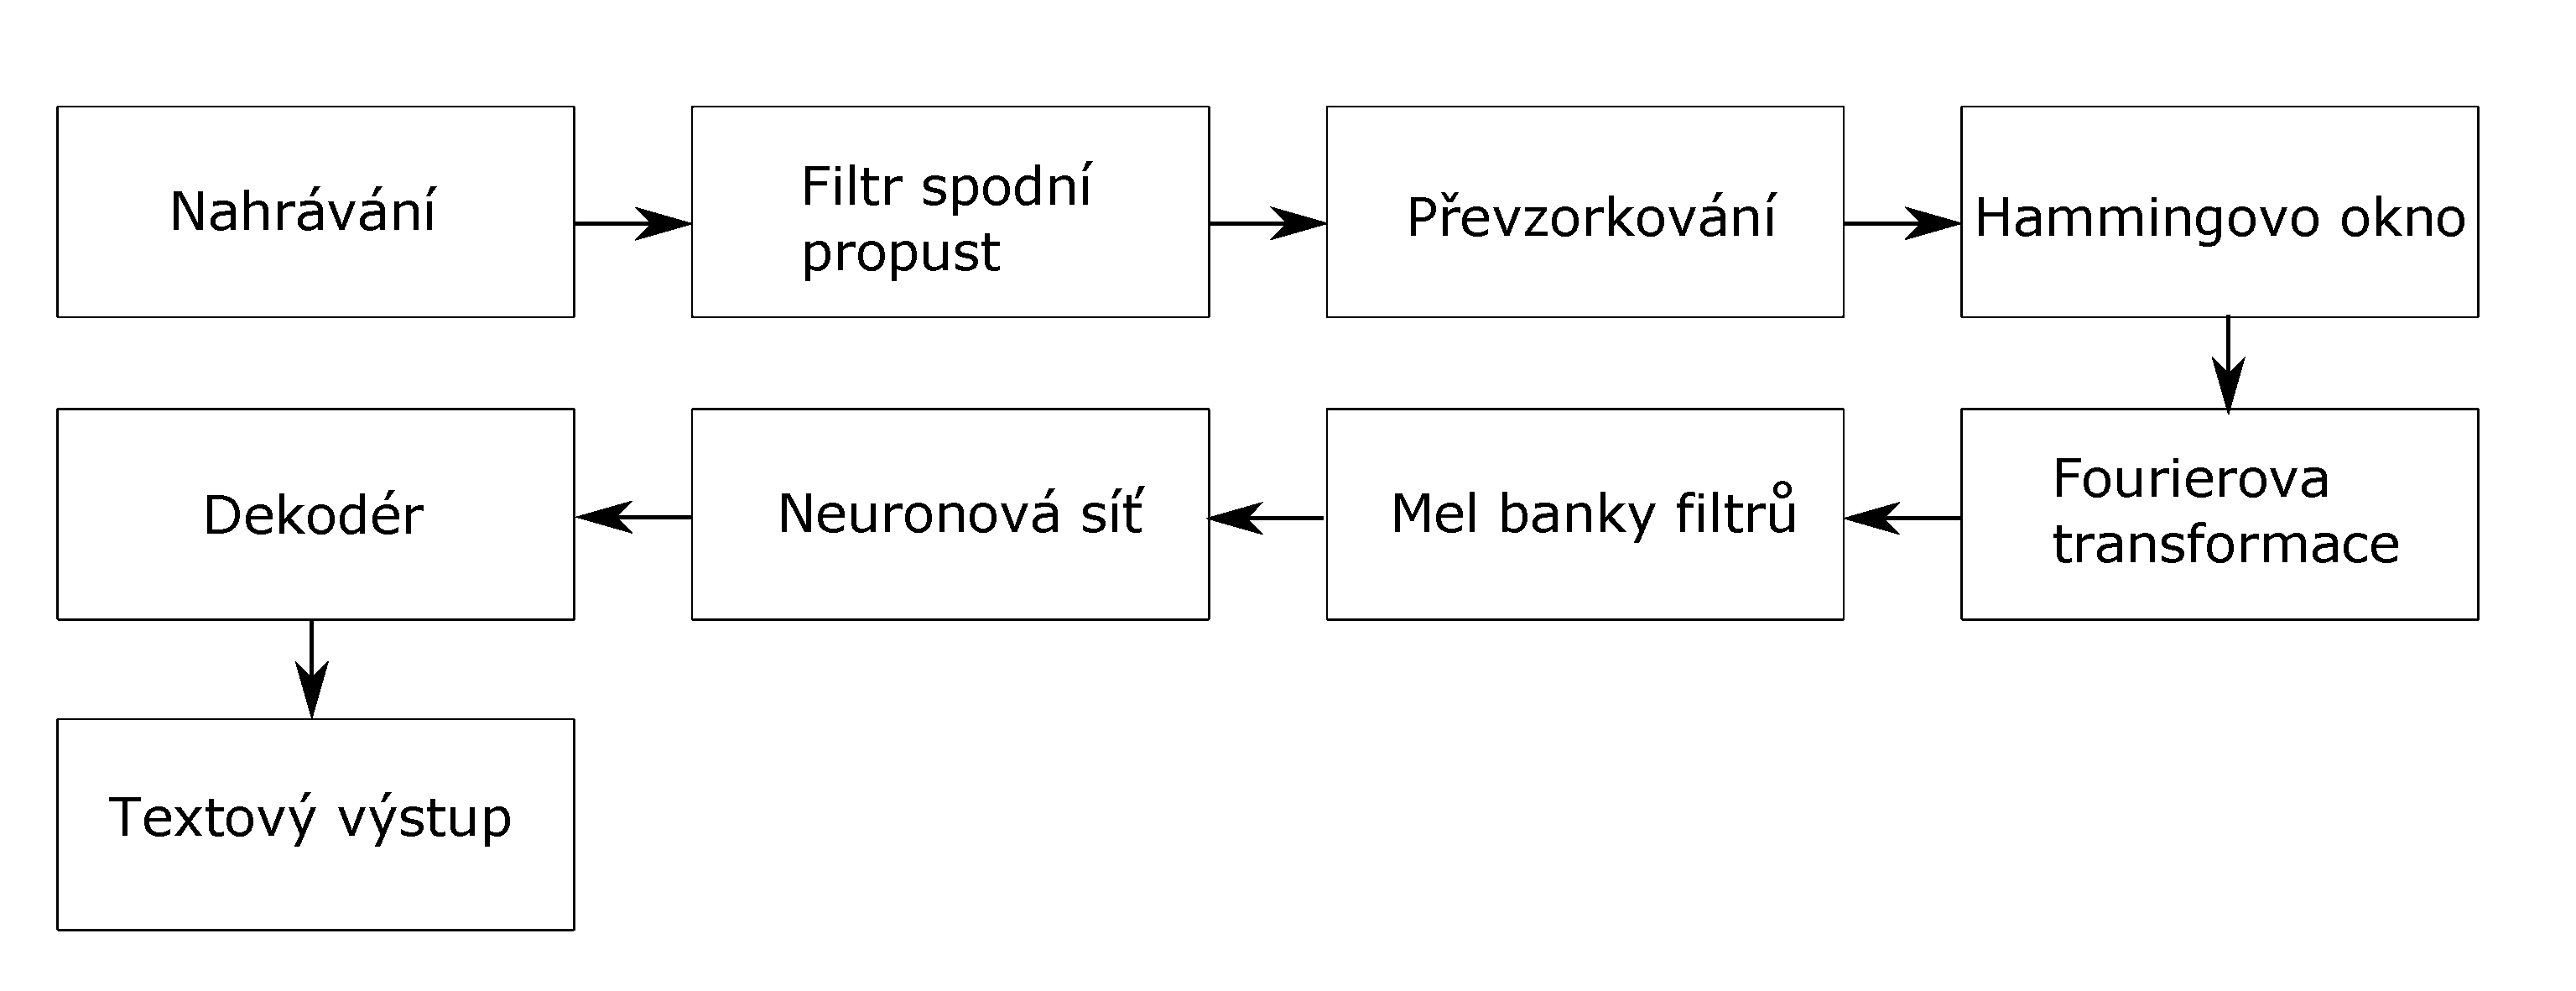
\includegraphics[height=6cm]{obrazky-figures/data_flow.pdf}
        \caption{Kroky zpracování signálu řeči}
        \label{fig:data_flow}
\end{figure}
Jsou zde uvedeny základní informace o~způsobu uložení signálu v~diskrétních zařízeních a udává informace o~správných krocích pro uložení signálu řeči a jeho předzpracování před extrakcí příznaků. Dále je zde popsán postup extrakce příznaků pro rozpoznávání řeči pomocí Mel bank filtrů a techniky využité k~její následné klasifikaci za využití neuronové sítě. Poslední část kapitoly vysvětluje princip dekodéru, jazykového a akustického modelu a také popisuje zpracování spojité řeči.

\newpage
\section{Zvukový signál}
Zvukový signál je reprezentací vibrací vzduchu či jiného přenosového média buď analogovou nebo digitální formou. 
\subsection{Digitální reprezentace}
Zvuk je v~běžných zařízení nahráván analogově, ale abychom byli schopni ho ukládat v~paměti a dále s~ním nějak pracovat, je nutné ho převést do diskrétní podoby. Toho je dosaženo za pomocí vzorkování spojitého signálu, jehož zdrojem může být například mikrofon v~mobilním zařízení, s~využitím analogově digitálního převodníku. 
\begin{figure}[H]
	\centering
		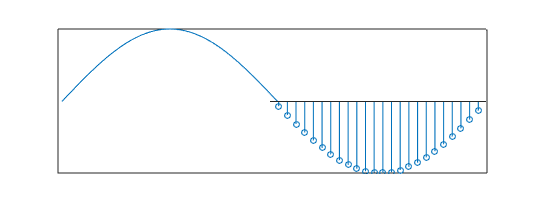
\includegraphics[height=6cm]{obrazky-figures/discrete_continuous_signal.png}
        \caption{Porovnání spojitého a diskrétního signálu}
\end{figure}
Přímo v~paměti je běžně jeden vzorek digitálního signálu uložen jako 8 bitů či jejich násobek, to se nazývá bitová hloubka. Hodnota vzorku určuje amplitudu signálu v~určitém okamžiku. 

Další vlastností je vzorkovací frekvence. Ta definuje, kolik vzorků audia je v~jedné sekundě záznamu.

Také je možné signál reprezentovat v~mono nebo stereo formátu. Stereo umožňuje uložení zvuku tak, aby se posluchači mohlo zdát, že zvuk přichází z~určitého směru, ovšem, v~případě reálně nahrávaného zvuku, je nutné využití dvou mikrofonů. Proto, že v~rozpoznávání řeči by tohle přineslo více nevýhod než výhod, např. dvojnásobné množství dat ke zpracování, je vhodnější data nahrávat pouze na jeden kanál.

\subsection{Řeč}
Vzhledem k~tomu, že cílem je rozpoznávání řeči a ne jiného druhu zvukového signálu, je možné výrazně omezit, které frekvence a jejich kombinace jsou pro nás podstatné.

Rozsah frekvence zvuku vydávaného lidským řečovým ústrojím se, u~průměrného člověka, pohybuje v~rozmezí 300~Hz až 3400~Hz. Díky tomu není nutné pro přenos signálu řeči používat vyšší frekvence. I~když v~krajních případech může omezení šířky frekvenčního pásma vést k~horšímu přenosu některých zvuků - např. hlásky "s"~a "f"~mohou znít v~telefonním pásmu (4~kHz) posluchači stejně \cite{human-hearing}.
\subsection{Převzorkování}
Běžně používanou vzorkovací frekvencí pro rozpoznávání řeči je 8000~Hz. Tato frekvence je využívána z~důvodu urychlení zpracování dat - data pro účely rozpoznávání zachovávají dostatečnou kvalitu řeči v~signálu (dáno Shannonovým teorémem popsaným níže), ale výrazně snižuje množství dat ke zpracování \cite{rabiner2011theory}. Další důvod využití této frekvence je historický, jelikož byla a stále je používána pro signál přenášený v~telefonické komunikaci

Zpravidla je ovšem většina zvukových záznamů nahrávána ve vyšší frekvenci, je proto nutné snížit vzorkovací frekvenci záznamu. Toho je dosaženo pomocí převzorkování.

Před převodem z~vyšších frekvencí je ovšem vhodné použít filtr dolní propust. Po aplikaci dolní propusti je z~původního signálu odebrán každý N-tý vzorek, kde N je podílem původní vzorkovací frekvence a frekvence požadované.
\subsubsection{FIR filtr - dolní propust}
Filtr s~konečnou odezvou je diskrétní lineární filtr, který se v~konečném čase ustálí na hodnotě 0. V~této implementaci je využit pro aplikaci filtru dolní propust při převzorkování za účelem odstranění nechtěných frekvencí a vyhnutí se aliasingu signálu. Spodní propust ponechává v~signálu pouze frekvence pod určitou úrovní, proto je využit k~izolaci mluveného slova. FIR filtr lze vyjádřit rovnicí \ref{eq:fir_filter}
\begin{equation} \label{eq:fir_filter}
\begin{gathered}
y[n] = \sum^{N}_{k=0}{h[k]x[n-k]}\\
\text{ kde $x$ je vstupní signál, $h$ je impulzní odezva, $y$ je výstupní signál a N je řád filtru}
\end{gathered}
\end{equation}

\subsubsection{Shannonův teorém}
Tento teorém udává, že vzorkovací frekvence signálu musí být dvakrát větší, než nejvyšší frekvence, kterou chceme přenášet. Proto je v~našem případě využita vzorkovací frekvence 8~kHz. V~případě nedodržení tohoto pravidla dochází v~signálu k~aliasingu a kvalita informací v~něm přenášených je výrazně snížena.

\section{Extrakce příznaků}
Extrakce příznaků je obecně v~rozpoznávání proces zaměřený na snížení množství dat nutných k~jejich klasifikaci, tedy výraznému snížení dimenzionality vstupních dat. Menší množství dat velmi urychluje proces rozpoznávání a šetří cenný procesorový čas. Dále extrakce poskytuje možnost se zbavit irelevantních dat a soustředit se pouze na ty, co jsou nezbytné. 
\subsection{Segmentace}
Prvním krokem při zpracování zvukového signálu pro extrakci příznaků je segmentace. Vstupem této části je audio signál, jehož předzpracování bylo popsáno v~předchozí podkapitole.  

Signál je nutné rozdělit na malé části, aby bylo možné určit, v~jakém stavu bylo v~daný moment řečové ústrojí člověk (např. vyslovení hlásky "a"). Tyto části jsou nazývány rámce. Běžná délka rámce je 20-25 milisekund a jejich překryv má velikost 10-15 ms. 

\begin{figure}[H]
	\centering
		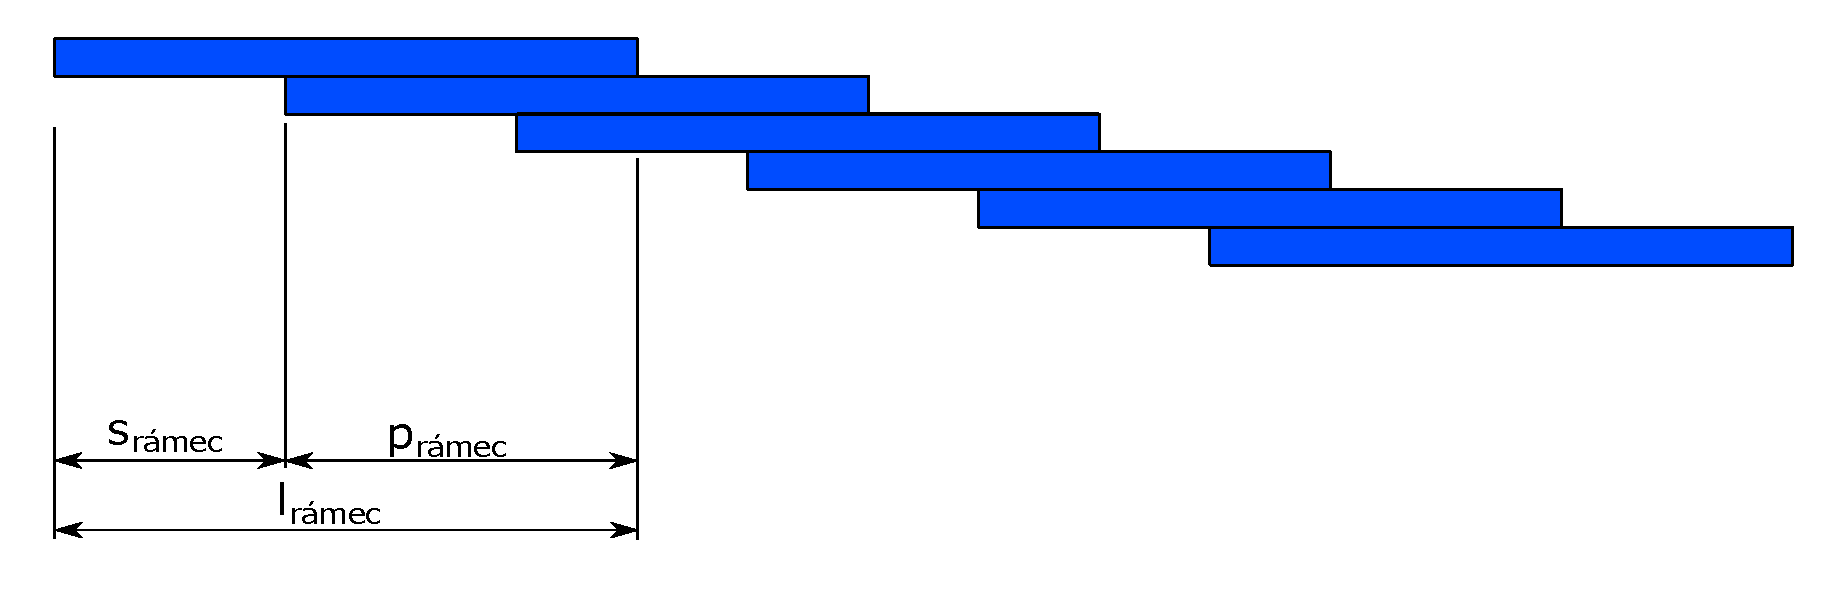
\includegraphics[height=4.8cm]{obrazky-figures/frames.pdf}
        \caption{Reprezentace rámců - $l_{ramec}$ - délka rámce, $s_{ramec}$ - posun, $p_{ramec}$ - překryv}
\end{figure}


Specificky v~této implementaci je délka rámce 25 ms a překryv 15 ms.
\subsubsection{Okenní funkce}
\label{sec:window_function}
Po rozdělení signálu na části je na každý rámec aplikována okenní funkce.  Důvodem jejich využití je získání lepších výsledků při použití Fourierovy transformace.
 V~této implementaci je využito Hammingovo okno. Tato funkce oslabuje amplitudu signálu na okrajích rámce.
 
\begin{equation}
w(n) = \alpha - \beta \cos(\dfrac{2\pi n}{N - 1}) \text{ kde }\alpha = 0.54, \beta = 0.46
\end{equation}

\begin{figure}[H]
	\centering
		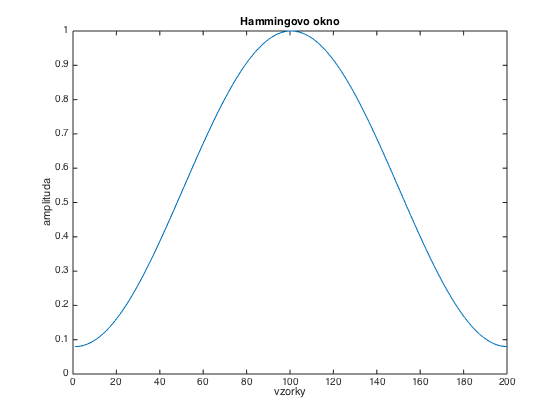
\includegraphics[height=6cm]{obrazky-figures/hamming_window.png}
        \caption{Hammingovo okno}
\end{figure}

\subsection{Fourierova transformace}
Fourierova transformace umožňuje rozdělení vstupního signálu na periodické frekvence, ze kterých je složen. Díky tomu můžeme zjistit, ve kterých frekvencích má signál nejvíce energie. Jelikož každý tón vydávaný lidským hlasovým ústrojím má svoje specifické frekvenční složky, je jejich rozložení nesmírně důležité pro jejich automatizované rozpoznávání \cite{9780073039381}.

\begin{equation}
	X_k=\sum_{n=0}^{N-1}x_ne^{\frac{-i2\pi kn}{N}}
\end{equation}

\subsubsection{Rychlá Fourierova transformace}
FFT je speciální verzí Diskrétní Fourierovi transformace, která je široce využívaná pro její výpočet. Oproti DFT, jejíž složitost je $O(N^2)$, dosahuje FFT složitosti $O(N\log N)$, což výrazně snižuje dobu výpočtu.
\subsection{Mel bank filtry}
Vstupem mel bank filtrů je Fourierova transformace jednotlivých rámců signálu. Pomocí trojúhelníkových okenních funkcí jsou energie v~každé části spektra namapovány na mel měřítko. Po výpočtu funkcí je každá z~nich logaritmizována a tyto hodnoty se využívají v~dalších výpočtech.

Parametry okenních funkcí použitých pro výpočet energií jsou závislé na počtu použitých filtrů, ze kterých chceme počítat energii, vzorkovací frekvenci signálu a velikosti vstupních dat. Také je možné dále omezit frekvence, které nás nezajímají tím, že změníme počáteční frekvenci nejnižšího okna, respektive konečnou frekvenci okna nejvyššího
.
\begin{figure}[H]
	\centering
		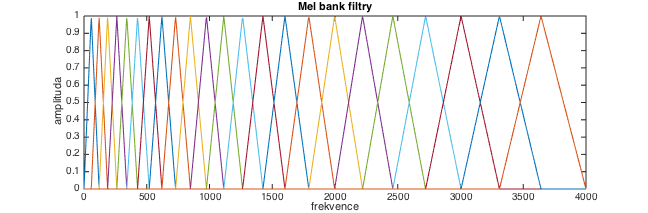
\includegraphics[height=4cm]{obrazky-figures/mel_bank_filters.png}
        \caption{Mel bank filtry - 24 filtrů, vzorkovací frekvence 8~kHz}
\end{figure}

Výstupem je matice logaritmů energií v~signálu. Tímto jsme dosáhli podstatného snížení dimenzionality oproti původním datům. Po vypočtení energií je každý kanál normalizován pomocí odečtení průměru energií v~daném kanálu přes celou nahrávku za účelem normalizace energie mluvy řečníka.

\begin{figure}[H]
	\centering
		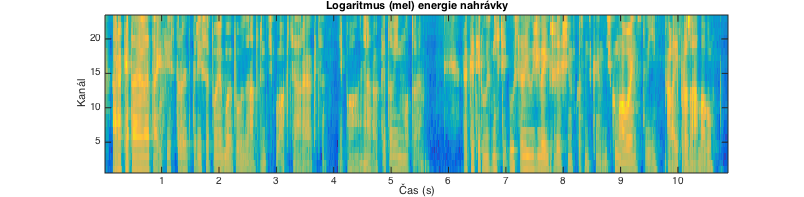
\includegraphics[height=4cm]{obrazky-figures/log_mel_power.png}
        \caption{Matice logaritmu energií nahrávky}
\end{figure}

\subsubsection{Mel měřítko}
Člověk, v~porovnání s~počítačem, vnímá zvukové frekvence řeči rozdílně. Posluchači by se mohlo zdát, že rozdíl frekvencí je výrazně nižší, než ve skutečnosti. Se zvyšující se frekvencí je tento jev výraznější \cite{1937ASAJ....8..185S}.

Mel měřítko vzniklo přesně z~tohoto důvodu, aby bylo možné lépe aproximovat jakým způsobem člověk ve skutečnosti zvuk vnímá. Převod mezi frekvencí a mel je prováděn pomocí rovnice \ref{eq:f_to_mel}. Pro převod z~mel měřítka do frekvence je možné použít rovnici \ref{eq:mel_to_f}.

\begin{equation}
m=2595\log_{10}(1+\frac{f}{700})=1127\ln(1+\frac{f}{700})
\label{eq:f_to_mel}
\end{equation}

\begin{equation}
	f=700(10^{\frac{m}{2595}}-1)=700(e^{\frac{m}{1127}}-1)
    \label{eq:mel_to_f}
\end{equation}

\section{Neuronová síť} \label{sec:nn}
Neuronové sítě jsou využívány jako nástroj, který se dokáže na základě trénovacích dat naučit klasifikovat vstupní data. Specificky v~rozpoznávání řeči mohou být použity přímo pro její rozpoznání nebo, jako v~případě této práce, pro extrakci příznaků.

\subsection{Struktura}
Neuronové sítě se skládají z~částí - neuronů - které provádí základní matematické operace. Každý neuron má na svém vstupu jednu nebo více hodnot. Množství těchto hodnot závisí na typu sítě a její velikosti. 

Typ sítě, který je pro tuto práci podstatný je tzv. feedforward. Tento typ je nejjednodušším typem neurální sítě. Jeho vrstvy jsou striktně odděleny a informace se v~něm mohou pohybovat pouze jedním směrem - tedy od vstupních uzlů k~výstupním.   

Vrstvy se dělí na tři typy. Prvním z~nich je vrstva vstupní. Ta na vstup přijímá data určená ke klasifikaci - v~našem případě výstup Mel bank filtrů. Vrstva zpracuje data a předá je tzv. skryté vrstvě. Těchto vrstev může být virtuálně neomezené množství. Poslední typ, výstupní vrstva, udává výsledek klasifikace. Počet výstupních uzlů určuje kolik různých tříd je síť schopna klasifikovat. V~případě rozpoznávání řeči mohou být výstupem např. pravděpodobnosti tzv. phoneme posteriors, tedy klasifikace fonémů řeči. Vizualizace jednoduché neuronové sítě je na obrázku \ref{fig:nn_layers}. 

\begin{figure}[H]
	\centering
		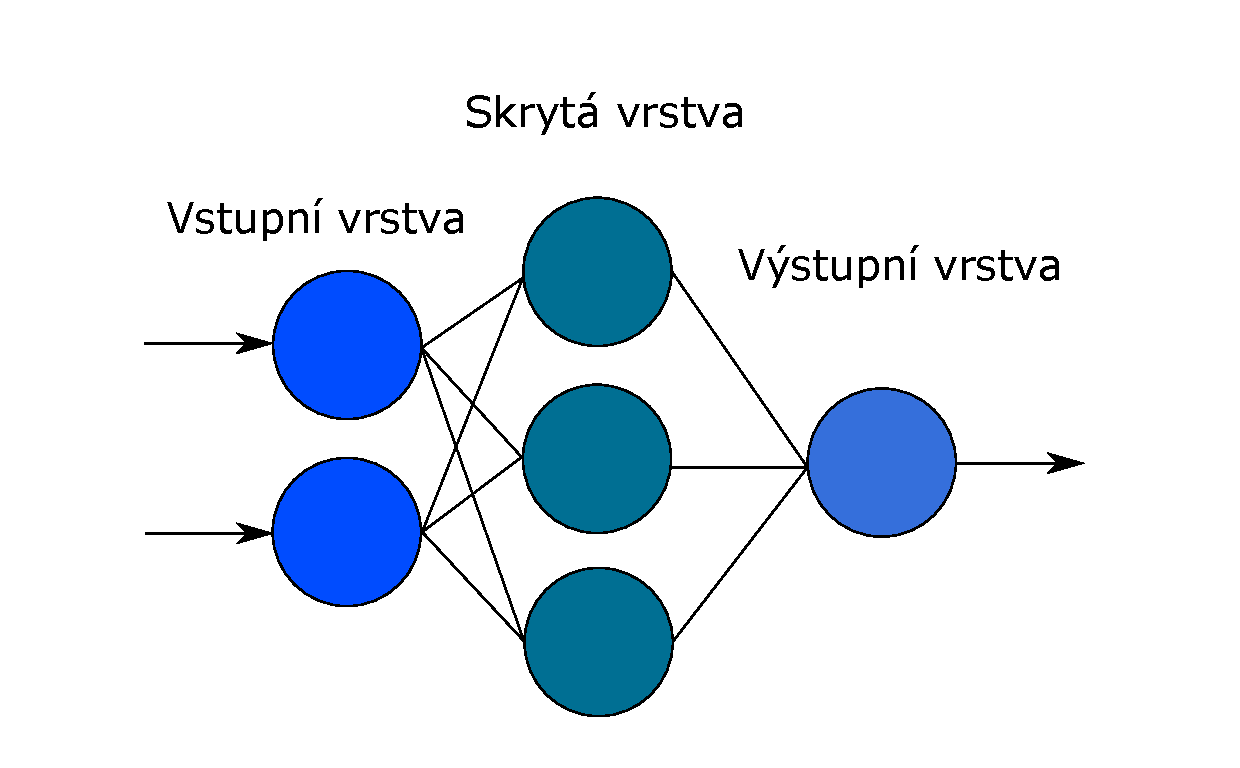
\includegraphics[height=5cm]{obrazky-figures/nn_layers.pdf}
        \caption{Grafická reprezentace jednoduché neuronové sítě}
        \label{fig:nn_layers}
\end{figure}

\subsubsection{Neuron}
Neuron je základní výpočetní jednotkou sítě. Na úrovni vstupní vrstvy každý neuron odpovídá jedné části vstupních dat. Na svůj vstup přijímá součet všech spojení na něj napojených z~předchozí vrstvy (rovnice \ref{eq:neuron_function}) a - v~některých implementacích - k~nim přičítá tzv. bias. Ke každému ze zmíněných spojení je přiřazena váha, kterou je přenášená hodnota vynásobena. Po sečtení dat je výsledek odeslán do aktivační funkce. Nejběžnější z~nich je sigmoidální přenosová funkce - rovnice \ref{eq:activation_function}.

\begin{equation}
	f(x)=\frac{1}{1+e^{-x}}
    \label{eq:activation_function}
\end{equation}

\begin{equation} \label{eq:neuron_function}
\begin{gathered}
out_i=S(\sum_{i=1}^{N}(\omega_ix_i) + \Theta) \\
\text{ kde $x$ je vstup neuronu, $\omega$ je váha spojení, $\Theta$ je bias a $S()$ je aktivační funkce }
\end{gathered}
\end{equation}
\begin{figure}[H]
	\centering
		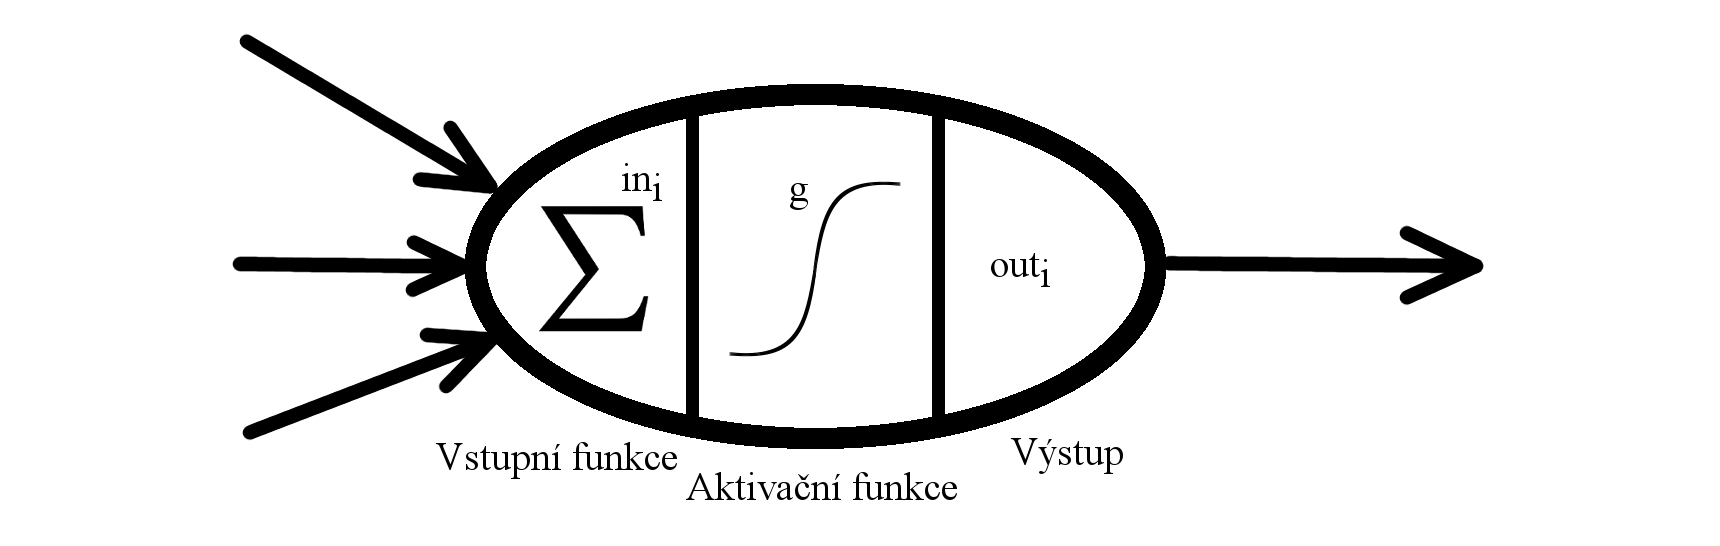
\includegraphics[height=4cm]{obrazky-figures/nn_neuron.png}
        \caption{Grafická reprezentace neuronu}
\end{figure}
\subsubsection{Dopředná neuronová síť}
Typ sítě využitý v~této práce se nazývá dopředná neuronová síť (feed forward). Jedná se o~nejjednodušší a zároveň také nejběžněji využívaný způsob implementace. Data v~síti prochází pouze jedním směrem a síť obsahuje obvykle alespoň jednu skrytou vrstvu. Zpravidla bývají všechny uzly sousedních vrstev propojeny. Grafická reprezentace malé sítě tohoto typu je zobrazena na obrázku \ref{fig:nn_layers}.

\newpage
\section{Dekodér}\label{sec:decoder}
Účelem dekodéru je nalezení nejpravděpodobnější sekvence slov $\tilde{W}$ podle pozorované sekvence příznaků $O$. Vzhledem k~velké varianci toho, jak mohou být slova vyřčena různými řečníky (například různá délka mluvy, barva hlasu nebo přízvuk) není možné jednoznačně určit, které slovo bylo vyřčeno. Tento problém je ilustrován na obrázku \ref{fig:one_analog} a je z~něj jasné, že ani jeden řečník nevysloví slovo nikdy stejně, proto jsou využity dále popsané metody. Informace uvedené v~této podkapitole byly čerpány z~\cite{psutka}.
\begin{figure}[H]
	\centering
		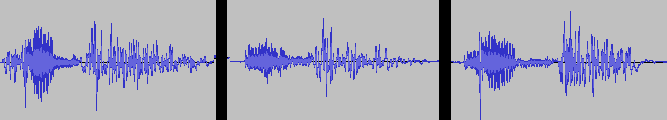
\includegraphics[height=2cm]{obrazky-figures/one_analog.png}
        \caption{Slovo "one"~třikrát vyřčeno stejným řečníkem}
        \label{fig:one_analog}
\end{figure}

Rovnice \ref{eq:decoder_prob} popisuje jakým způsobem je získána nejpravděpodobnější posloupnost slov \~{W}. Cílem je tedy na základě pozorovaných příznaků $O$ nalézt posloupnost slov, která jim nejlépe odpovídá, tedy $P(W|O)$.
\begin{equation} \label{eq:decoder_prob}
\begin{gathered}
\tilde{W} = \underset{W}{\mathrm{arg max}} P(W|O) 
\end{gathered}
\end{equation}

Aplikací Bayesova pravidla získáme rovnici \ref{eq:decoder_bayes}. Tato úprava umožňuje rozdělení problému do několika částí, které lze modelovat odděleně. První z~nich je apriorní pravděpodobnost výskytu slov $P(W)$, která reprezentuje jazykový model (\ref{sec:language_model}), druhou je pravděpodobnost $P(O|W)$ jenže nese informaci o~akustickém modelu (\ref{sec:acoustic_model}). Hodnoty používané pro výpočet těchto pravděpodobností je nutné znát před samotným rozpoznáváním, je tedy nutné je natrénovat pomocí textových a řečových dat. Pravděpodobnost $P(O)$ nemá žádnou spojitost s~hledaným slovem $W$ a proto není při výpočtech využívána. Namísto toho je pro hledání slov použita rovnice \ref{eq:decoder_simplified}.

\begin{equation} \label{eq:decoder_bayes}
\begin{gathered}
\tilde{W} = \underset{W}{\mathrm{arg max }} \frac{P(W)P(O|W)}{P(O)}
\end{gathered}
\end{equation}

\begin{equation} \label{eq:decoder_simplified}
\begin{gathered}
\tilde{W} = \underset{W}{\mathrm{arg max }} P(W,O) = \underset{W}{\mathrm{arg max }} P(W)P(O|W)
\end{gathered}
\end{equation}

\subsection{Akustický model}\label{sec:acoustic_model}
Akustický model je používán k~reprezentování vztahů mezi zvukovým signálem a fonémy nebo jinými jednotkami, ze kterých je řeč složena. Je vytvářen za pomocí zvukových nahrávek a jejich přepisů. Jeho cílem je získat co nejlepší odhad podmíněné pravděpodobnosti $P(O|W)$ (rovnice \ref{eq:decoder_simplified}). 

Základním předpokladem akustického modelování je to, že při mluvě je lidské řečové ústrojí v~dostatečně malém časovém rozsahu v~jednom z~konečného počtu stavů. Díky tomu je možné rozdělit slova na malé jednotky určené těmito stavy - v~tomto případě fonémy.

Jak již bylo zmíněno v~předchozí sekci, klasifikaci výstupu Mel bank filtrů obstarává neuronová síť, jejímž výstupem jsou pravděpodobnosti jednotlivých fonémů. Tyto pravděpodobnosti jsou zpracovány v~dekodéru, kde jsou jednotlivé výslovnosti slov modelovány pomocí Markovových modelů.

\subsubsection{Skryté Markovovy modely}
Nejpoužívanějším způsobem akustického modelování jsou v~současné době skryté Markovovy modely (Hidden Markov Models). Jedná se o~o~model stochastického procesu, který generuje v~diskrétních časových okamžicích vektor pozorování $O$ a zároveň také mění svůj stav podle pravděpodobností přechodů $a_{ij}$. Pravděpodobnosti přechodu určují s~jakou pravděpodobností přechází model ze stavu $s_i$ do stavu $s_j$. Tato pravděpodobnost je definována rovnicí \ref{eq:a_calc}. Zároveň jsou tyto pravděpodobnosti v~modelu konstantní, nemění se tedy s~časem a jejich součet je jedna (rovnice \ref{eq:hmm_a_sum}).

\begin{equation} \label{eq:a_calc}
\begin{gathered}
a_{ij} = P(s(t+1) =s_j|s(t) = s_i)
\end{gathered}
\end{equation}

\begin{equation} \label{eq:hmm_a_sum}
\begin{gathered}
\sum_{j=1}^{N}a_{ij} = 1
\end{gathered}
\end{equation}

Při zpracování řeči jsou používány modely, ve kterých lze vyjádřit časový posun. Vzhledem k~tomu, že jsou data zpracována po rámcích, reprezentuje přechod jeden časový krok. Ukázka takového modelu je vyobrazena na obrázku \ref{fig:simple_hmm}.

\begin{figure}[H]\label{fig:simple_hmm}
	\centering
		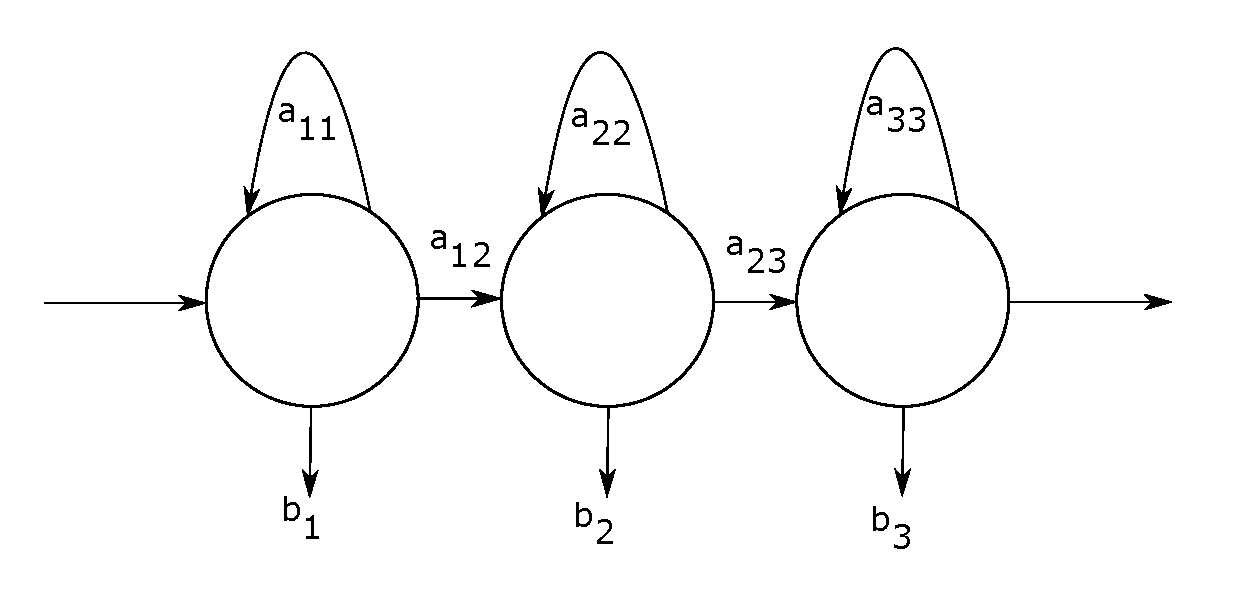
\includegraphics[height=4cm]{obrazky-figures/simple_hmm.pdf}
        \caption{Jednoduchý Markovův model}
\end{figure}

Konečným výstupem akustického modelu je vektor pravděpodobností výskytu modelovaných jednotek.

\subsection{Jazykový model}\label{sec:language_model}
Jazykový model obsahuje slovník, který určuje, jaká slova rozpoznávač podporuje a také obsahuje pravidla pro zřetězení zmíněných slov. Důvodem jeho využití je tedy co nejpřesnější odhad $P(W)$ pro rozpoznávanou posloupnost slov (rovnice \ref{eq:decoder_simplified}). Tuto pravděpodobnost je možné vyjádřit vztahem v~rovnici \ref{eq:lm_words}. 

\begin{equation} \label{eq:lm_words}
\begin{gathered}
P(W) = \prod^{k}_{i = 0}P(w_i)
\end{gathered}
\end{equation}

Předchozí rovnice ovšem popisuje pouze výpočet pravděpodobnosti pro unigramový jazykový model - tedy model, který definuje pouze pravděpodobnost výskytu jednotlivých slov. Tento model samozřejmě zlepšuje přesnost rozpoznávání, ovšem běžně používané jazykové modely obsahují n-gramy vyššího řádu.

N-gramy definují pravděpodobnost výskytu slova na základě historie $n - 1$ slov. Rovnice \ref{eq:lm_words_bigram} popisuje výpočet za využití bigramů, tedy pravděpodobnost výskytu slova závisí na jednom předchůdci. To, že pravděpodobnost závisí pouze na historii nám umožňuje provádět rozpoznávání již během promluvy a ne až po jejím skončení.

\begin{equation} \label{eq:lm_words_bigram}
\begin{gathered}
P(W) = \prod^{k}_{i = 1}P(w_i | w_{i - 1})
\end{gathered}
\end{equation}

Model ovšem nemusí nutně obsahovat záznamy o~všech slovních kombinacích. Vzhledem k~tomu, že není možné získat dostatek trénovacích dat na pokrytí všech kombinací, je v~bigramových modelech a modelech vyššího řádu využívána tzv. backoff pravděpodobnost. Ta zajišťuje, že kombinacím, které nebyly nalezeny, není přiřazena nulová pravděpodobnost. V~případě nenalezení záznamu pro bigram je použita rovnice \ref{eq:lm_words_bigram_backoff}.

\begin{equation} \label{eq:lm_words_bigram_backoff}
\begin{gathered}
P(w_i|w_{i - 1}) = P(w_i)B(w_{i - 1})
\end{gathered}
\end{equation}

Kde $P(w_i)$ je unigramová pravděpodobnost a $B(w_{i - 1})$ je backoff pravděpodobnost předcházejícího slova.
\subsection{Rozpoznávání spojité řeči}\label{sec:continuous_speech}
Rozpoznávání spojité řeči s~sebou oproti rozpoznávání izolovaných slov přináší jisté problémy. Rozpoznávač izolovaných slov funguje poměrně přímočaře - modelem jsou posílány získané příznaky a všechny informace z~modelu vystupující, krom těch, které zůstanou na konci, jsou odstraněny. V~případě rozpoznávání spojité řeči to ovšem není tak jednoduché a je nutné provádět mezislovní přechody.

\begin{figure}[H]\label{fig:continuous_speech}
	\centering
		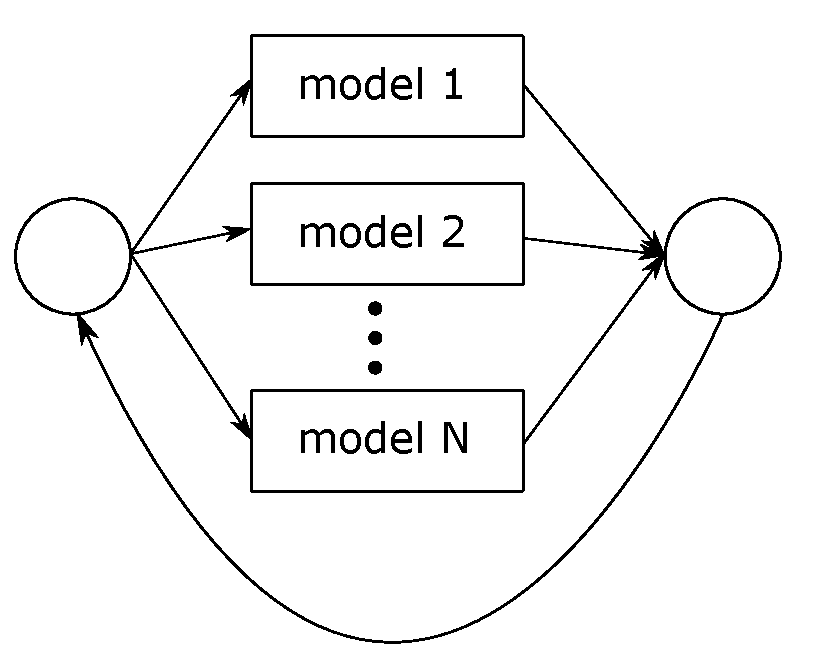
\includegraphics[height=4cm]{obrazky-figures/continuous_speech_model.pdf}
        \caption{Rozpoznávací síť pro spojitou řeč. Jednotlivé modely reprezentují slova v~síti, N je počet slov.}
\end{figure}

Obrázek \ref{fig:continuous_speech} zobrazuje jednoduchý model pro spojitou řeč. Jednotlivé vnitřní modely reprezentují slova ve slovníku rozpoznávače. Na místě výstupu je tzv. mezislovní přechod, který posílá informace zpět na začátek modelu. Kvůli tomu je zvýšena jak paměťová (je nutné ukládat historii slov, kterými se v~průchodu modelem prošlo), tak i výpočetní náročnost.

\chapter{Implementace}
Tato kapitola popisuje implementaci rozpoznávače řeči. Seznamuje čtenáře s~technologiemi využitými v~programu, externími knihovnami a funkcemi nutnými pro chod aplikace. Kapitola také obsahuje popis struktury knihovny a informace o~jejím rozhraní. Vysvětluje, jakým způsobem byly vytvořeny jednotlivé části rozpoznávače. Pro maximalizaci rychlosti výpočtu je celý proces implementován v~NDK, tedy jazyku C++ a v~Renderscriptu.

\section{Použité technologie}
Společnost Google, která je vývojářem otevřené platformy Android, poskytuje vývojářům několik různých nástrojů pro tvorbu jejich aplikací. Využité nástroje pro implementaci projektu jsou popsány v~této podkapitole.

\subsection{Android Studio}
Android Studio je oficiálním vývojovým prostředím (dále IDE) pro platformu Android. Je založen na IDE IntelliJ IDEA od firmy JetBrains. Podporuje nejpoužívanější operační systémy, tedy Windows, macOS a Linux. 

Toto IDE podporuje jak vývoj v~Javě, na Androidu nejpoužívanějším jazyku, tak i v~nativním prostředí, tedy C++ nebo C. Dále také obsahuje nástroje pro tvorbu uživatelského rozhraní, které byly použity pro tvorbu demonstrační aplikace

\subsection{Android NDK}
Z~důvodu neoptimální rychlosti interpretace bytecode pod Androidem je vývojářům umožněno psaní nativního kódu přeloženého specificky pro architektury využívané v~mobilních zařízeních. 

Překlad nativního kódu je v~Android Studio prováděn za pomoci nástroje CMake, případně ndk-build. Ndk-build je ovšem podporován jen z~důvodu zpětné kompatibility se staršími projekty. V~tomto projektu byl využit CMake.

\subsection{JNI}\label{sec:jni}
Java Native Interface definuje způsob, jakým kód napsaný v~Javě interaguje s~nativním kódem psaným v~C++. Umožňuje tedy připravit rozhraní pro nativní kód.

\subsection{Renderscript}
Renderscript\footnote{\url{https://developer.android.com/guide/topics/renderscript/compute.html}} je jazyk založený na standardu C99 jazyka C. Je určen pro spouštění výpočetně náročných operací. Hlavní silou Renderscriptu je jeho soustředění na paralelizaci a velkou výhodou v~tomto směru je to, že paralelizace je řízena systémem. Díky tomuto je kód v~něm napsaný přenositelný. Zároveň může Renderscript runtime zadat některé části výpočtu i GPU zařízení.

I~přes to, že hlavním účelem vytvoření Renderscriptu bylo urychlení zpracování grafických operací, je možné ho využít i pro naše účely. Je to velice užitečný nástroj jak pro paralelizaci extrakce příznaků, tak i pro zrychlení výpočtu neuronové sítě.

Pro generování C++ tříd pro použití skriptů je použit Gradle, ovšem pro překlad zdrojového kódu je nutné využít ndk-build.

\subsection{OpenSL ES}
OpenSL je multi-platformní knihovnou pro zpracování zvukového signálu. Dodává nástroje pro zaznamenání a přehrání zvuku a mnoho dalších vlastností, které v~tomto projektu nejsou podstatné. 

V~NDK se nachází poněkud ošizená verze této knihovny, pro účely této implementace jsou ale její funkce dostatečné. Hlavní nevýhodou této verze je zbytečně složité používání v~nativním kódu.

\subsection{Git}
Git je verzovací systém využíván pro týmový vývoj. I~přes to, že je tento projekt vypracováván samostatně, je Git velice užitečným nástrojem. Využívám ho převážně pro zálohu zdrojových kódů na vzdáleném serveru a také pro jeho přenos mezi zařízeními.

Jako hostovací server pro svoje úložiště jsem zvolil GitHub\footnote{\url{https://github.com}} kvůli předchozích zkušenostem s~tímto serverem ať už pro osobní nebo školní projekty.

\section{Externí knihovny a funkce}

\subsection{FIR filtr}
Pro aplikaci filtru dolní propusti jsem využil třídy Filter\footnote{\url{https://cardinalpeak.com/blog/a-c-class-to-implement-low-pass-high-pass-and-band-pass-filters/}}. Tato třída implementuje tři základní filtry pro zpracování zvukové stopy - dolní, horní a pásmovou propust. Pro převzorkování vstupního zvukového záznamu je v~programu využit pouze filtr dolní propust. Zdrojový kód je distribuován pod modifikovanou BSD licencí.

\subsection{KissFFT}
KissFFT\footnote{\url{http://kissfft.sourceforge.net/}} je velmi malá knihovna pro výpočet FFT(Rychlá Fourierova Transformace) napsaná v~jazyce C. Byla vybrána z~důvodu jednoduchosti jejího použití a naprosto dostatečné rychlosti výpočtu. Knihovna je distribuovaná pod modifikovanou BSD licencí.

\section{Struktura knihovny}
Program je tvořen jako knihovna pro použití v~Android SDK. Pro použití v~jiných aplikací tedy němu tedy tvořené žádné grafické rozhraní, slouží pouze pro použití v~nějakém větším celku, např. aplikace pro ovládání zařízení za pomocí hlasových příkazů. 

Zdrojové kódy knihovny jsou děleny do logických celků, z~nichž každý zastává jeden úkol. Následuje popis jednotlivých částí a důležitých tříd v~nich obsažených. Diagramy třídy jsou v~příloze \ref{app:class_diag}.

\paragraph{Feature\_extraction} Obsahuje třídy obstarávající extrakci příznaků (příloha \ref{app:feature_extraction}). Třída \texttt{AudioFrame} poskytuje metody pro operace nad rámci audio signálu. Dále také obsahuje třídy \texttt{RSMelFilterBank} a \texttt{RSNeuralNetwork}, které využívají Rendescript k~aplikaci Mel bank filtrů a výpočtu neuronové sítě.

\paragraph{Voice\_Activity\_Detection} Pouze třída \texttt{VoiceActivityDetector} pro detekci řečové aktivity (příloha \ref{app:voice_activity_detection}).

\paragraph{Decoder} Složka s~definicemi tříd pro dynamický dekodér (příloha \ref{app:decoder}). Hlavní třídou tohoto balíčku je \texttt{ViterbiDecoder}, která zaobaluje funkce všech ostatních tříd. Dále je zde obsažena třída \texttt{HMMGraph}, která definuje strukturu rozpoznávací sítě a také třída \texttt{Token} reprezentující tokeny algoritmu Token Passing.

\paragraph{Threads} Zahrnuje třídy pro vlákna a komunikaci mezi nimi a dále také callbacky do virtuálního prostředí Javy (příloha \ref{app:threads}).

\paragraph{Utility} Třídy s~různými účely, např. čtení WAV souboru nebo nahrávání audio signálu (příloha \ref{app:utility}).

Dále je zde obsažena třída \texttt{SpeechRecognitionAPI} poskytující rozhraní pro využívání knihovny. Umožňuje programátorovi využít možnosti nahrávání a současného rozpoznávání zvukového signálu nebo signálu z~WAV souboru. Obdobná třída je implementována i v~Javě. Obě tyto rozhraní využívají návrhového vzoru observer pattern\footnote{\url{http://w3sdesign.com/?gr=b07\&ugr=proble}} pro notifikaci posluchačů o~změnách v~rámci rozpoznávání (změna detekované aktivity řeči, rozpoznání věty a dokončení rozpoznávání).

\section{Nahrávání a zpracování zvukové stopy}
Pro nahrávání zvukového signálu jsem využil knihovnu OpenSL. Audio je nahráváno do bufferu ve vzorkovací frekvenci 48~kHz a v~bitové hloubce 16~bitů. Při nahrání určité délky nahrávky, v~tomto případě délka překryvu rámce, tedy 10 ms, je vyvolán callback a data jsou předána do vlákna pro extrakci příznaků.

Po předání dat je signál převzorkován na požadovanou frekvenci - 8~kHz. Dále je převeden z~datového typu short int na float, jelikož další části rozpoznávače pracují s~reálnými čísly. 

\subsection{Zpracování ze souboru}
V~případě zpracování ze souboru je proces poněkud jednodušší. Jediné operace, které je nutné vykonat je kontrola formátu vstupního souboru. Tato implementace podporuje pouze soubory uložený ve formátu WAV, které splňují následující požadavky: vzorkovací frekvence musí být 8~kHz, audio obsahuje pouze jeden kanál (mono nahrávka), bitová hloubka je 16 bitů a uložená data jsou ve formátu PCM.

Následné zpracování probíhá obdobně jako při nahrávání. Do vlákna extrakce příznaků je odesílán signál rozdělený na části o~délce 10 ms.
\section{Extrakce příznaků}\label{sec:impl_fe}
Extrakce je prováděna souběžně s~nahráváním zvuku. V~prvotních fázích implementace nebylo možné provádět kompletní extrakci zároveň s~nahráváním, ovšem po využití průběžné normalizace energií popsané níže byla tato limitace odstraněna.

Segmentace zvukového signálu je částečně řešena za pomoci callback funkce, kterou vyvolává vlákno pro nahrávání audio signálu, jelikož je předána délka záznamu odpovídající délce překryvu jednotlivých rámců. Pro účely uložení dat rámce a jeho další zpracování je vytvořena třída AudioFrame.

Dalším krokem extrakce je aplikace Hammingova okna (\ref{sec:window_function}). Jedná se o~jednoduchou operace násobení, kterou není nutné nijak optimalizovat. Koeficienty okna je nutné počítat pouze jednou a to při inicializaci rozpoznávače.

Následuje aplikace Rychlé Fourierovy transformace. Knihovna KissFFT přijímá na vstup rámec signálu a vrací výsledek FFT o~určité délce. Vstupní data transformace mají délku 256 vzorků - jedná se o~rámec signálu (200 vzorků) a 56 nulových hodnot.

Všechny tyto kroky jsou implementovány v~již zmíněné třídě AudioFrame. Ta v~sobě uchovává dílčí výsledky a uvolňuje paměť v~momentě, kdy už data nejsou potřebná.

Následujícím, výpočetně náročnějším krokem je výpočet mel bank filtrů. K~akceleraci výpočtu je využit Renderscript. Díky Rendersriptu je každý kanál mel bank počítán paralelně a rychlost výpočtu je výrazně vyšší, než při sekvenčním výpočtu. Aplikaci mel bank filtrů obstarává třída RSMelFilterBank. Aplikace jednoho filtru se řídí algoritmem \ref{alg:mel_filter}, je implementována v~Renderscriptu a zpracování všech filtrů mel bank může potenciálně běžet souběžně.

\begin{center}
\begin{czechalgorithm}[H] \label{alg:mel_filter}
\SetKwFunction{FMelFilter}{MelFilter}
\SetKwProg{Fn}{Function}{:}{}

    \Fn{\FMelFilter{$index\_filtru$, $fft\_vstup$}}{
        \For{$i\leftarrow 0$ \KwTo $\text{Délka FFT dat}$}{
            result = result + mel\_filtry[index\_filtru][i] * (fft\_vstup[i].real + fft\_vstup[i].imaginary)
        }
        \eIf{result < 1}{
          result = 0
        }{
          result = log(result)
        }
        \KwRet result;
    }
 \caption{Aplikace mel filtru}
\end{czechalgorithm}
\end{center}


Parametry jednotlivých filtrů jsou počítány před zahájení extrakce a tento výpočet není nutné opakovat. Po aplikaci všech filtrů jsou výsledky odeslány do detektoru řečové aktivity, který je popsán v~následující sekci. 

Normalizace získaných dat probíhá pouze na rámcích detekovaných jako aktivní a je řešena odečtením celkového průměru v~jednotlivých filtrech, tedy:

\begin{equation} \label{eq:mel_normalisation}
\begin{gathered}
y_n = x_n - \sum^{n - 1}_{i = 0}h_i
\end{gathered}
\end{equation}

Kde $x_n$ je vstup, $y_n$ je výstup a $h$ jsou předchozí vstupy. Průměr samozřejmě není v~každém kroku vypočítán na základě všech předchozích dat, ale je využíván tzv. klouzavý průměr (angl. moving average, rovnice \ref{eq:moving_average}).

\begin{equation} \label{eq:moving_average}
\begin{gathered}
AVG_{n + 1} = \frac{n\cdot AVG_{n} + x_{n + 1}}{n + 1}
\end{gathered}
\end{equation}

Kde $AVG_{n + 1}$ je nový průměr, $n$ je počet zprůměrovaných hodnot, $x_{n + 1}$ je nová hodnota pro výpočet.

\section{Detekce řečové aktivity}\label{sec:imple_vad}
Důvody pro využití detekce řečové aktivity jsou dva. Prvním z~nich je zlepšení normalizace řečníka, která je popsána v~předchozí kapitole. Druhým důvodem je možnost deaktivovat výpočet neuronové sítě a dekodér v~časových okamžicích, ve kterých není mluva detekována. To samozřejmě výrazně snižuje časovou náročnost zpracování.

Samotná detekce je implementována poměrně jednoduchým způsobem. Aktivita je určována podle výstupů mel bank filtrů, tedy energií nahrávky v~určitých částech spektra. V~případě, že je součet všech logaritmů energií nižší než 0, je rámec považován za ticho. Formální popis je v~rovnici \ref{eq:vad}.

\begin{equation} \label{eq:vad}
\begin{gathered}
f(\vec{n}) =
  \begin{cases}
    true       & \quad \text{jestli }\sum^N_{i = 0} n_i > 0\\
    false  & \quad \text{jinak} 
  \end{cases}
\\
\text{kde N je velikost vstupního vektoru a n je vstupní vektor}
\end{gathered}
\end{equation}

Určení aktivity pouze pro jednotlivé rámce by ovšem nebylo dostatečné. Často by docházelo k~tomu, že za aktivní segmenty by mohly být považovány i velmi malé časové úseky. Proto detektor umožňuje nastavit hranice, kterými je určen minimální časový limit pro přechod z~jednoho stavu do druhého. Vhodné hodnoty byly zjištěny experimentálně. Pro přechod ticho$\rightarrow$řeč se ukázala vhodnou hodnota 7 rámců a pro přechod řeč$\rightarrow$ticho 25 rámců.

Z~důvodu zpožděných přechodů detektor obsahuje vlastní zásobník předchozích rámců, které jsou dále využity v~případě přechodu do aktivního stavu. Pokud by tento zásobník nebyl implementován, mohlo by docházet k~velké ztrátě informací.

\section{Klasifikace}\label{sec:imple_nn}
Klasifikace dat na fonémy je implementována prostřednictvím neuronové sítě. Již natrénovaná neuronová síť mi byla dodána vedoucím práce, proto v~této práci není její trénování pokryto. Tato neuronová síť byla trénovaná na trénovací sadě TED-LIUM pocházející z~Kaldi receipe \cite{Rousseau2014EnhancingTT}. 

\begin{table}[H]
\centering
\caption{Parametry neuronové sítě}
\label{tab:nn_params}
\begin{tabular}{|l|l|l|}
\hline
Vrstva & Velikost & Aktivační funkce \\ \hline
Vstup  & 360      & -                \\ \hline
1      & 500      & sigmoida         \\ \hline
2      & 500      & sigmoida         \\ \hline
3      & 80       & -                \\ \hline
4      & 500      & sigmoida         \\ \hline
5      & 46       & softmax          \\ \hline  
\end{tabular}
\end{table}

Síť používá jako aktivační funkci sigmoidu popsanou v~podkapitole \ref{sec:nn}. Pouze třetí, bottleneck, vrstva nevyužívá žádné aktivační funkce. Na konečný výstup sítě je aplikována funkce softmax pro normalizaci výstupních hodnot (rovnice \ref{eq:softmax}). Jelikož dekodér pracuje s~logaritmy pravděpodobností, je při výpočtu výsledek funkce softmax zlogaritmován.

\begin{equation} \label{eq:softmax}
\begin{gathered}
y_n = \frac{\exp(x_n)}{\sum^N_{i = 0}\exp(x_i)}
\end{gathered}
\end{equation}

\begin{figure}[H]
	\centering
		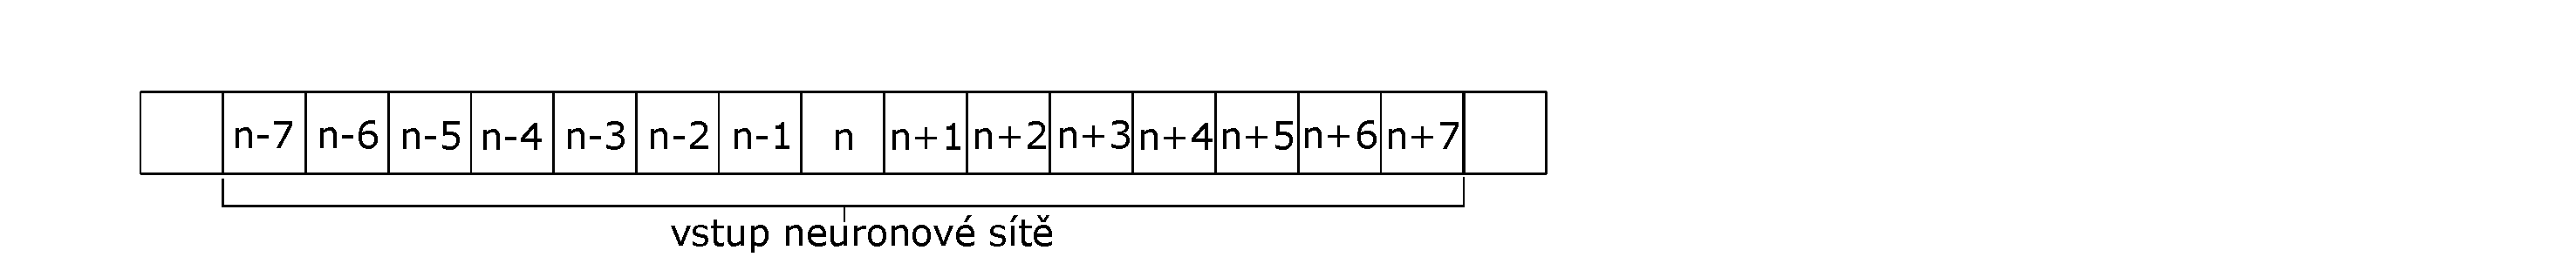
\includegraphics[height=2.2cm]{obrazky-figures/nn_input.pdf}
        \caption{Vstupní data neuronové sítě}
\end{figure}

Vstupem sítě jsou výsledky mel bank filtrů. Z~matice výsledků jsou postupně brány jednotlivé rámce a jejich okolí -- přesněji 7 rámců. V~případě, že některé rámce nejsou dostupné (např. při začátku promluvy) je vícekrát využit první resp. poslední dostupný rámec. Data je dále také nutné přeorganizovat, jelikož síť očekává, že kanály jednotlivých mel bank budou přímo následovat.

Samotná síť je implementována ve třídě RSNeuralNetwork. K~urychlení výpočtu je opět využit Renderscript. Bohužel v~současné verzi Renderscriptu není možné interně synchronizovat vlákna, proto bylo nutné algoritmus sítě rozdělit do více částí, jinak by mohlo dojít k~desynchronizaci dat a výsledky výpočtu by byly nekonzistentní -- výpočet další vrstvy by mohl začít předtím, než se připraví data z~vrstvy předchozí. Při výpočtu výstupů každé vrstvy je tedy nutné za pomocí NDK čekat na dokončení výpočtu. Data ovšem není nutné kvůli tomuto nijak zpracovávat a mohou zůstat v~prostředí Renderscriptu, takže tento proces nepřidává téměř žádnou režii. 

Paralelizace algoritmu neuronové sítě je řešena následujícím způsobem. Namísto výpočtu pomocí maticových operací jsou Renderscriptu předány hodnoty naučené sítě a dat pro zpracování a hodnoty jsou vypočteny pouze pro daný neuron. Poté je potenciálně pro každý neuron spuštěno jedno vlákno - záleží na tom, jak se Renderscript Runtime rozhodne práci rozdělit, tohle nemůže programátor nijak řídit. Oproti sekvenčnímu výpočtu v~C++ je tento přístup přibližně 5-krát rychlejší. Bližší informace o~srovnání rychlosti výpočtu lze nalézt v~podkapitole \ref{sec:comparison}.

\section{Dekodér}\label{sec:imple_dec}
Jak již bylo zmíněno v~podkapitole \ref{sec:decoder}, dekodér je implementován za využití skrytých Markovových modelů (dále HMM). HMM jsou reprezentovány formou stromu se zpětnými ukazateli. Každý uzel grafu tedy obsahuje ukazatele jak na všechny svoje přímé předchůdce, tak i přímé následovníky.

V~této implementaci je za účelem snížení paměťové náročnosti implementován dynamické dekodér. Ten, na rozdíl od dekodéru statického, vytváří pouze unigramovou rozpoznávací síť a získává hodnoty n-gramových pravděpodobností z~jazykového modelu uloženého paměti ve vyhledávací struktuře, řešení uložení jazykového modelu je popsáno v~sekci \ref{sec:n_grams}. 

Každý uzel grafu v~sobě udržuje informace o~pravděpodobnostech přechodu do dalších stavů - přesněji logaritmy těchto pravděpodobností - dále také index výstupu neuronové sítě, který určuje jaký foném daný uzel přijímá na svém vstupu. Z~důvodu urychlení přístupu k~nejlépe hodnocenému tokenu je zde také obsažen ukazatel na nejlepší token. 

V~grafu jsou definovány dva uzly se speciálním účelem. První z~nich je počáteční uzel, ten slouží k~předávání tokenů vstupním stavům jednotlivých slov. Druhým je výstupní uzel, ten je využit pro přidání záznamu Word link record (\ref{sec:word_link_record}) a výpočtu $P(W)$. Zjednodušená grafická reprezentace grafu je na obrázku  \ref{fig:one_hmm_sil}.

\begin{figure}[H]\label{fig:one_hmm_sil}
	\centering
		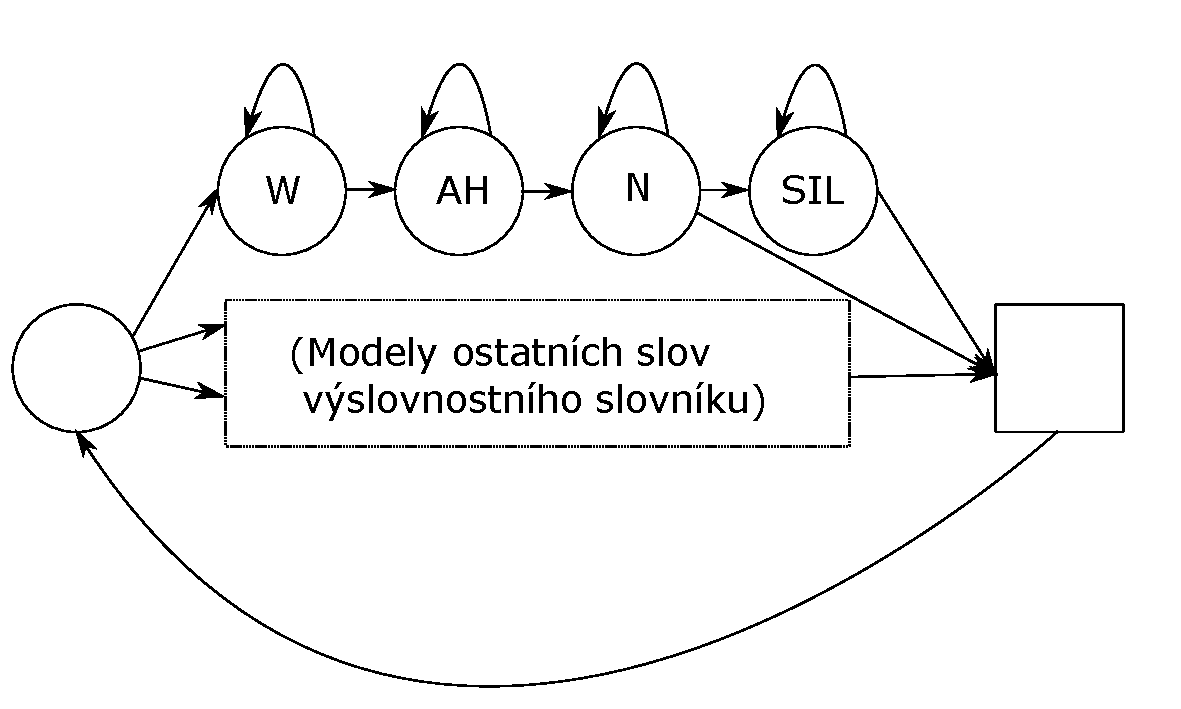
\includegraphics[height=6cm]{obrazky-figures/hmm_network.pdf}
        \caption{Grafická reprezentace rozpoznávací sítě se slovem "one" a přidaným SIL na konec slova}
\end{figure}

Celý graf je vytvořen při inicializaci rozpoznávače na základě slovníku a jazykového modelu uloženého v~paměti zařízení. Pro každé slovo je na konec přidán alternativní uzel přijímací na svém vstupu pravděpodobnost výskytu ticha. Lepším řešením by pravděpodobně bylo přidat na výstup všech slov sdílený uzel přijímající ticho, jelikož tokeny v~každém uzlu SIL již nepřijmou před výstupem do dalšího slova žádný jiný foném. Tím by se dal snížit počet stavů HMM grafu o~počet slov ve slovníku a o~stejné množství i počet aktivních tokenů.

\subsection{Token passing}
Token passing je široce využívaným algoritmem pro zjištění nejpravděpodobnější cesty skrze HMM. Lze jej využívat jak pro rozpoznávání izolovaných slov nebo, jako v~případě této práce, pro spojitou řeč. Popis lze nalézt v~algoritmu \ref{alg:token_passing}. Popis algoritmu byl převzat z~článku \cite{YoungN1989TokenP}.

\begin{center}
\begin{czechalgorithm}[H] \label{alg:token_passing}
	\textbf{Inicializace:}\\
    Počáteční stavy modelu obsahují token s~ohodnocením 0;\\
    Ostatní stavy obsahují token s~nekonečnou cenou.\\
    \textbf{Algoritmus:}\\
    \For{$t\leftarrow 0$ \KwTo $T$}{
    	\ForEach{stav i}{
        	Nakopíruj token ze stavu $i$ do všech napojených stavů a přepočítej jeho ohodnocení.
        }
        Odstraň původní tokeny.\\
        \ForEach{stav i}{
        	Najdi ve stavu $i$ token s~nejlepším ohodnocením a odstraň zbytek.
        }
        \ForEach{výstupní stav i}{
        	Vytvoř nový záznam Word link record pro každý aktivní stav $i$.\\
            Navaž záznam na ten uložený v~tokenu.\\
            Změň ukazatel cesty tokenu na tento nově vytvořený záznam.\\
        }
    }
    
    \textbf{Výsledek:}\\
    Z~výstupních stavů vyber nejlépe ohodnocený token. Tento token určuje nejpravděpodobnější cestu grafem.
 \caption{Token passing}
\end{czechalgorithm}
\end{center}

Velmi důležitou částí tohoto algoritmu je tzv. \textbf{Viterbiho kritérium}. To udává, že v~rámci jednoho stavu lze uchovat pouze token s~nejlepším ohodnocením a ostatní zahodit. Tokeny s~horším ohodnocením nemohou být v~dalších krocích nikdy hodnoceny lépe, než ten momentálně nejlepší a proto by byl jejich výpočet zbytečný. 

V~první verzi dekodéru byly tokeny implementovány jako objekty, které se při každém přechodu v~paměti alokovaly a dealokovaly. Tento přístup se ukázal být velmi neefektivní kvůli vysoké režii, která tím byla do programu uvedena. Z~tohoto důvodu bylo nutné tento problém vyřešit jinak.

Ve finální verzi jsou v~rámci každého uzlu grafu alokovány tokeny již při vytvoření rozpoznávacího grafu a to tak, že pro každý uzel je vytvořeno tolik tokenů, kolik je do stavu vedeno přechodů. Díky tomu mohou být tokeny uchovány v~paměti neustále, i když to způsobuje vyšší paměťovou náročnost. Namísto vymazání tokenu (jak aplikací Viterbiho kritéria tak i pruningu) je pouze nastaven příznak neaktivity. Tento přístup vyžaduje procházení grafem od konce, jelikož nové hodnoty tokenů závisí na předcházejících uzlech. Díky tomuto přístupu je také možné aplikovat Viterbiho kritérium již po dokončení výpočtu v~každém uzlu, jelikož nově vypočtené hodnoty nejsou v~tomto kroku dále využity.

Všechny pravděpodobnosti jsou v~rozpoznávači reprezentovány jejich logaritmy pro možnost využití rychlého sčítání namísto pomalého násobení (rovnice \ref{eq:log_calc}). Po dokončení výpočtu není nutné logaritmy opět převádět do běžných pravděpodobností, stačí vybrat ten nejlépe ohodnocený.

\begin{equation} \label{eq:log_calc}
\begin{gathered}
\log(P_1 P_2) = log(P_1) + log(P_2)
\end{gathered}
\end{equation}

\subsubsection{Pruning}
S~využitím pruningu je možné opět snížit časovou náročnost programu. Pruning, podobně jako Viterbiho kritérium, umožňuje deaktivaci těch tokenů, které mají malou šanci na úspěch, alespoň v~daném časovém okamžiku. Nevýhodou jeho využití je ovšem možnost deaktivace tokenů, jež mohou v~dalších krocích získat lepší ohodnocení. Něco takového ovšem nelze předvídat. Typy pruningu využité v~této implementaci jsou \textbf{beam pruning} a \textbf{live states pruning}. Popis vykonání pruningu je v~algoritmu \ref{alg:pruning}.

\begin{center}
\begin{czechalgorithm}[H] \label{alg:pruning}
\SetKwFunction{FApplyPruning}{ApplyPruning}
\SetKwProg{Proc}{Procedure}{:}{}
	\tcc{Seznam "aktivní tokeny"~obsahuje všechny aktivní tokeny po aplikaci Viterbiho kritéria}
    \Proc{\FApplyPruning{}}{
   		Seřaď aktivní tokeny podle jejich ohodnocení, od nejlepšího.\\
        \tcp{beam pruning}
        hranice = ohodnocení nejlepšího tokenu + konstanta beam pruningu\\
        \ForEach{aktivní token t}{
            Pokud je ohodnocení tokenu t nižší než hranice, deaktivuj ho.
        }
        \tcp{live states pruning}
		Deaktivuj všechny tokeny krom N nejlepších.
    }
 \caption{Pruning}
\end{czechalgorithm}
\end{center}

\subsubsection{Word link record} \label{sec:word_link_record}
Důležitou součástí rozpoznávání spojité řeči pomocí token passingu je vhodné uložení historie slov pro výpočet $P(W)$. V~prvotní fázi jsem využíval objektů z~knihovny STL\footnote{\url{http://en.cppreference.com/w/cpp/container}}, tento přístup se ovšem osvědčil jako velice neefektivní. V~některých případech bylo nutné kopírovat kompletní historii a to způsobovalo velkou režii. Proto je historie ve finální verzi implementována za pomocí word link record.

Word link record v~principu funguje jako jednosměrně vázaný seznam, ovšem pouze zpětně. Jednotlivé záznamy slov jsou reprezentovány nezávislými objekty. Pro každý token procházející slovním přechodem je vytvořen nový záznam a je navázán na poslední záznam uložený v~daném tokenu. Záznamy v~historii mohou být sdíleny v~historii více tokenů, jak je vidět na obrázku \ref{fig:word_link_record} -- každý záznam bez příchozího ukazatele je poslední v~historii a je posledním záznamem v~některém z~tokenů. 

\begin{figure}[H]\label{fig:word_link_record}
	\centering
		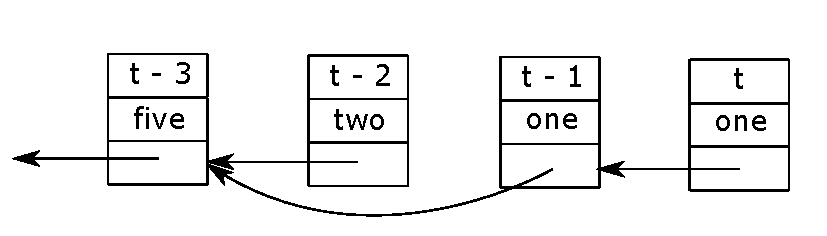
\includegraphics[height=2.6cm]{obrazky-figures/word_link_record.pdf}
        \caption{Příklad provázání word link record}
\end{figure}

Po dokončení rozpoznávání lze snadno zpětným průchodem záznamy zjistit, kterými slovy token s~nejlepším ohodnocením prošel. Kvůli usnadnění dealokace již nevyužívaných záznamů obsahuje každý objekt počítadlo referencí. World link record se tedy sám vymaže z~paměti poté, co již není v~historii žádného tokenu.

\subsection{N-gramy} \label{sec:n_grams}
Jak již bylo zmíněno v~\ref{sec:language_model}, v~této implementaci jsou pro jazykový model využity n-gramy. Specificky jsou podporované jazykové modely s~bigramy. Informace o~jazykovém modelu jsou uloženy v~souboru formátu ARPA\footnotetext{\url{http://www.speech.sri.com/projects/srilm/manpages/ngram-format.5.html}}.

Při inicializaci rozpoznávače jsou N-gramy načteny ze souboru uloženého v~paměti zařízení. Pro rychlejší přístup k~potřebných datům je každé slovo reprezentováno svým ID, tedy indexem, pod kterým se nachází ve vektoru všech slov. To zajišťuje přímý přístup do paměti při hledání daného slova. Každé slovo v~této struktuře využívá k~uložení bigramových pravděpodobností hashovací tabulku pro rychlé dohledání potřebného záznamu (opět podle ID slova). Hashovací tabulka sice zabírá více paměti než primitivnější způsoby uložení, ale výrazně snižuje dobu přístupu k~potřebnému záznamu. 

V~případě nenalezení bigramu v~hashovací tabulce je dohledána backoff pravděpodobnost předchozího slova přímým přístupem pomocí ID slova.

Ohodnocení přechodu mezi slovy je také měněno tzv. Word insertion penalty a je možné nastavit i škálování pravděpodobností n-gramů. Výpočet $P(w)$ se řídí rovnicí \ref{eq:fin_lm}.

\begin{equation} \label{eq:fin_lm}
\begin{gathered}
P(w_i) = P(w_i|w_{i - 1})\text{LM scale} + \text{word insertion penalty}
\end{gathered}
\end{equation}

\section{Vlákna}
Pro zrychlení výpočtu a využití více-jádrových CPU obsažených v~Android zařízeních je exekuce rozpoznávání rozdělena do několika vláken.

Prvním z~nich je vlákno, které dodává vstupní audio data. V~případě nahrávání z~mikrofonu se tedy jedná o~nahrávací vlákno, které předává každých 10 ms nahraného audio signálu. Čtení ze souboru funguje obdobným způsobem. Tato data jsou předávána do vlákna extrakce příznaků. Další vlákno obstarává extrakci příznaků (\ref{sec:impl_fe}) a detekci řečové aktivity(\ref{sec:imple_vad}) a posílá výsledek do vlákna neuronové sítě. Třetím vláknem je klasifikace za využití neuronové sítě (\ref{sec:imple_nn}) a posledním je samotný dekodér (\ref{sec:imple_dec}). 

\subsubsection{Předávání dat mezi vlákny}
Jelikož mezivláknová komunikace může způsobovat neočekávané chování, pokud není správně implementována, byla pro účely předávání dat vytvořena třída \texttt{SafeQueue}. Tato třída za pomocí zamykacích objektů (mutexů) umožňuje přístup k~objektu fronty pouze jednomu vláknu při souběžném přístupu. Dále tato třída využívá \texttt{std::condition\_variable} pro notifikaci vláken čekajících na další data. Tato implementace je inspirována návrhovým vzorem Producer/Consumer\footnote{\url{http://www.ni.com/white-paper/3023/en/}}. Zjednodušený diagram komunikace mezi vlákny je na obrázku \ref{fig:thread_comm}.

Typ předávaných dat se řídí výčtovým typem. Tyto typy jsou:
\begin{itemize}
\item DATA\quad-\quad audio data
\item INACTIVE\quad-\quad detekováno ticho
\item TERMINATE\quad-\quad konec vstupních dat, ukončení vláken
\end{itemize}

\begin{figure}[H]
	\centering
		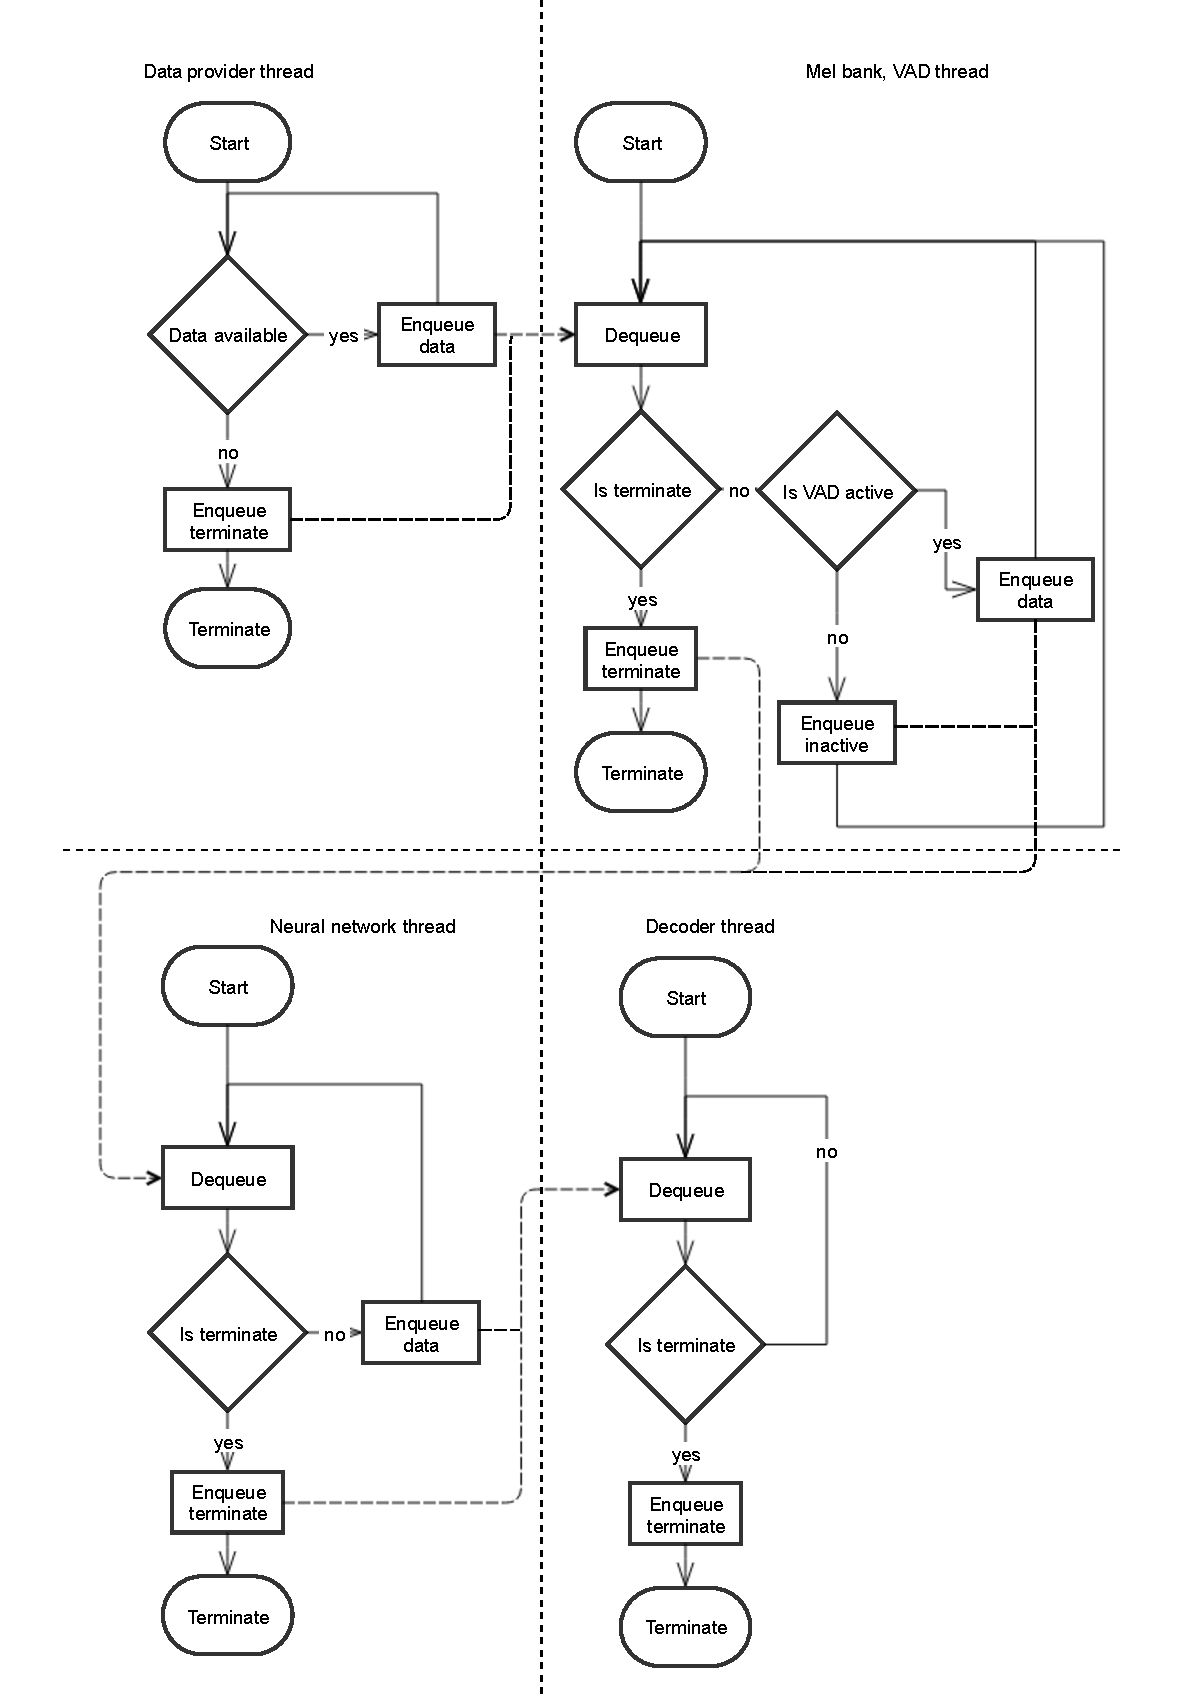
\includegraphics[height=20cm]{obrazky-figures/thread_communication.pdf}
        \caption{Zjednodušená grafická reprezentace mezivláknové komunikace}
        \label{fig:thread_comm}
\end{figure}

\subsection{Komunikace s~JVM}
Pro odesílání výsledků rozpoznávání a notifikování o~událostech, které v~kódu nastaly je nutné implementovat funkce, které dokáží předávat data z~nativního kódu do JVM. Pro tento účel byla využita knihovna JNI (\ref{sec:jni}). Při tvorbě rozpoznávače je uložena globální reference na objekt, který poskytuje rozhraní k~použití rozpoznávače. Tento objekt v~sobě obsahuje privátní metody, které jsou volány z~nativního kódu. Tímto způsobem je možné i předávat data pomocí parametrů funkcí tak, jak je běžné.

\section{Demo aplikace}
Pro účel předvedení funkčnosti rozpoznávače byla vytvořena jednoduchá Android aplikace. Tato aplikace umožňuje rozpoznávání jak přímým audio vstupem z~vestavěného mikrofonu zařízení, tak i z~audio nahrávek uložených v~jeho paměti. Cílem nebylo vytvořit aplikaci s~příjemným uživatelským rozhraním, ale spíše demonstrovat funkčnost a zobrazit důležité informace.

\begin{figure}[H]
	\centering
		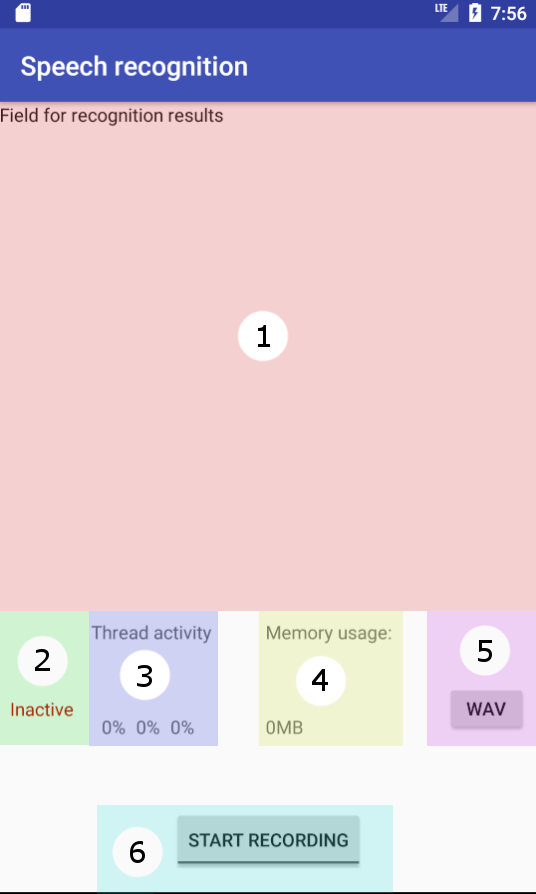
\includegraphics[height=8cm]{obrazky-figures/demo_app.png}
        \caption{Demo aplikace}
\end{figure}

UI aplikace se dělí na šest základních částí, následuje jejich popis:
\begin{enumerate}  
\item pole pro výsledky rozpoznávání,
\item aktuální stav detekce řečové aktivity,
\item aktivita jednotlivých vláken rozpoznávače (zleva mel bank filtry a detekce řečové aktivity, neuronová síť, dekodér),
\item aktuální využití paměti aplikací, včetně grafických prvků a paměti alokované v~JVM,
\item tlačítko pro demonstraci rozpoznávání z~WAV souboru,
\item tlačítko pro zapnutí/vypnutí nahrávání z~mikrofonu.
\end{enumerate}
Aplikace je lokalizována pro český a anglický jazyk a sama se přizpůsobí nastavení systému.

\chapter{Testování a vyhodnocení}
V~této kapitole je popsán proces verifikace výsledků implementovaných částí a srovnání implementací některých částí rozpoznávače v~jazycích Java, C++ a Renderscript. Také je zde obsaženo zhodnocení úspěšnosti rozpoznávání a vyhodnocení časových a paměťových nároků rozpoznávače.

Všechna měření v~této kapitole (krom hodnocení word error rate) byla prováděna na zařízení Lenovo A7020a48\footnote{\url{www.mobilespecs.net/phone/Lenovo/Lenovo_Vibe_K5_Note_A7020a48.html}}. Verze operačního systému Android na tomto zařízení je 6.0. Jedná se o~zařízení starší a střední cenové třídy, proto se dá předpokládat, že na novější zařízeních poběží rozpoznávač přinejmenším stejně rychle.

\section{Verifikace algoritmů}
Pro verifikaci výsledků jsem využil program MATLAB\footnote{\url{www.mathworks.com/products/matlab.html}} a funkce v~něm obsažené, případně skripty vytvořené komunitou. Dále byly výsledky porovnány s~referenční implementací dodanou vedoucím práce. Referenční kód byl dodán v~několika jazycích, pro srovnání jsem využil verze napsané v~jazycích Python a Java. 

Kód napsaný v~Javě bylo možné spuštět přímo na platformě Android a proto byl hlavním zdrojem kontrolních dat. Také tato implementace využívá datový typ float, díky čemuž výsledky lépe odpovídají této implementaci.

Algoritmy napsané v~C++ odpovídají výstupům referenční implementace, přesně podle očekávání. Implementace v~Renderscript ovšem vykazují jistou odchylku oproti referenčním výstupům i přes to, že je ve skriptech definována nejvyšší možná přesnost výpočtu. Odchylka je ale velmi malá, v~řádu desetin procent, tedy zanedbatelná. 

\section{Srovnání implementací}
\label{sec:comparison}
Srovnání rychlosti výpočtu bylo provedeno na dvou výpočetně nejnáročnějších částech extrakce příznaků - výpočet mel bank filtrů a neuronové sítě.

Pro účel srovnání rychlostí byla vytvořena audio nahrávka o~délce 11 sekund, převzorkovaná na vzorkovací frekvenci 8~kHz. Pro přesné údaje byl každý algortimus spuštěn 50x a na testovacím zařízení bylo spuštěno minimum procesů, které by mohly výsledky testů ovlivnit.

\begin{table}[H]
\centering
\caption{Rychlosti výpočtů}
\label{tab:speed_comp}
\begin{tabular}{|l|l|l|}
\hline
             & Mel banky filtrů & Neuronová síť \\ \hline
Java         & 1837 ms         & 22009 ms      \\ \hline
C++          & 447 ms          & 12223 ms      \\ \hline
Renderscript & 229 ms          & 2735 ms       \\ \hline
\end{tabular}
\end{table}

Jak je vidět v~tabulce \ref{tab:speed_comp}, rychlost výpočtu je v~nativním kódu výrazně vyšší než ve virtuálním prostředí Javy. Tohle samozřejmě není žádným překvapením. 

Pro srovnání rychlosti C++ a Renderscript slouží především výpočet mel bank filtrů. Vzhledem k~výraznému rozdílu jsem se rozhodl Renderscript použít i pro výpočet neuronové sítě, implementace v~C++ ovšem není příliš optimalizovaná a slouží spíše ke srovnání s~Javou.

Díky Renderscriptu je tedy možné provádět obě testované části - jak mel filtr banky, tak výpočet neuronové sítě - zároveň s~nahráváním zvukové stopy i bez výrazného zatížení CPU či GPU, pokud ho v~daném zařízení Renderscript Runtime využívá.

Srovnání rychlosti výpočtu neuronové sítě bylo prováděno na menší síti použité v~začátku vývoje pro srovnání s~referenční implementací.

\section{Hodnocení úspěšnosti rozpoznávání}
Pro hodnocení úspěšnosti byl využit tzv. word error rate (WER). Výpočet se řídí rovnicí \ref{eq:wer}. Pro výpočet WER jsem využil skriptu asr\_evaluation\footnote{\url{https://github.com/belambert/asr-evaluation}}.

\begin{equation} \label{eq:wer}
\begin{gathered}
WER = \frac{S~+ D + I}{N}
\end{gathered}
\end{equation}

Kde $S$ je počet substitucí, $D$ počet smazaných slov, $I$ počet vložených slov a $N$ je počet referenčních slov.

Přesnost rozpoznávače je tedy následně dána rovnicí \ref{eq:wacc}.
\begin{equation} \label{eq:wacc}
\begin{gathered}
WAcc = 1 - WER = \frac{N - S~- D - I}{N}
\end{gathered}
\end{equation}

Měření těchto hodnot bylo prováděno spouštěním extrakce příznaků přímo na Android zařízení, vzhledem k~využití Renderscriptu a nemožnosti tedy tuto část spustit na jiném operačním systému než Android. Kód dekodéru je ovšem implementován v~c++14 a pro ušetření času a možnosti využít většího slovníku než na mobilním zařízení. 

Velikost slovníku využita pro hodnocení:

\begin{table}[H]
\centering
\caption{Velikost slovníku}
\label{tab:lm_info}
\begin{tabular}{|l|l|l|}
\hline
unigramy & bigramy & výslovnostní slovník \\ \hline
10003    & 86128   & 12046   \\ \hline
\end{tabular}
\end{table}

Pro testovací data byla využita sada TED-LIUM obsahující nahrávky TED přednášek. Tato testovací sada obsahuje přibližně 3 hodiny nahrávek.

\newpage
Prvním experimentem bylo zjištění vhodné hodnoty pro word insertion penalty. Důvod využití této hodnoty je popsán v~\ref{sec:n_grams}. Pro testování byly zvoleny hodnoty v~intervalu $\langle0, -15\rangle$ s~krokem $1$ a škálovací koeficient jazykového modelu 1. Výsledky testů jsou v~obrázku \ref{fig:word_insertion_penalty}.

\begin{figure}[H]\label{fig:word_insertion_penalty}
\begin{center}
\begin{tikzpicture}
\begin{axis}[
	xlabel={word insertion penalty},
    y unit = \%,
    ylabel={word error rate}
]
\addplot table [x=WER, y=WIP, mark=none, color=red]{data/wip_wer.txt};
\end{axis}
\end{tikzpicture}
\end{center}
\caption{Vliv word insertion penalty na WER}
\end{figure}

Z~grafu vyplývá, že při nepoužití této konstanty je rozpoznávání na velice špatné úrovni. Rozpoznávač bez ní rozpoznává jako vhodná i velice krátká slova a výstup je prakticky nečitelný. Jako optimální se ukázala být hodnota $word\_insertion\_penalty = 8$ a ta je použita i v~následujících testech. Vyšší hodnoty vykazují mírné zhoršení kvality rozpoznávání.


Další experiment pokrývá nalezení vhodné hodnoty škálovacího koeficientu jazykového modelu. Otázkou je, zda-li je nutné tento koeficient vůbec používat. V~testech byly použity hodnoty z~intervalu $\langle0, 6.0\rangle$ s~krokem $0.1$. Nejvhodnější hodnotou se ukázalo být $4.1$.

\begin{figure}[H]
\begin{center}
\begin{tikzpicture}
\begin{axis}[
	xlabel={škálovací koeficient bigramových pravděpodobností},
    y unit = \%,
    ylabel={word error rate}
]
\addplot table [x=SCALE, y=WER, mark=none, color=red]{data/lm_scale_wer.txt};
\end{axis}
\end{tikzpicture}
\end{center}
\caption{Vliv škálování jazykového modelu na WER}
\end{figure}

Další změny parametrů již neměli žádný pozitivní vliv na kvalitu rozpoznávání. Průměrný word error rate rozpoznávače je tedy přibližně 80\%.

Jak již bylo zmíněno na začátku této sekce, velikost slovníku použita k~vyhodnocení obsahuje přibližně 10000 slov. Tento slovník sloužil především ke zhodnocení kvality samotného dekodéru, pro použití na mobilních zařízení je ale taková velikost slovníku pro tuto implementaci nereálná. Reálné hodnoty pro použití v~mobilních zařízeních jsou popsány v~následující sekci.

\section{Časová a paměťová náročnost}
Obrázek \ref{fig:cpu_activity} zobrazuje aktivity procesoru v~různých fázích rozpoznávání. Červená barva určuje část, ve které probíhá pouze detekce řečové aktivity (a k~tomu nutný výpočet mel filtrů). Z~grafu je jasně vidět, že tato část má minimální nároky na procesor. Modrá část zobrazuje začátek zpracování dat pomocí neuronové sítě při detekování řečové aktivity před samotnou aktivací dekodéru. Zeleně vyznačená oblast kombinuje jak extrakci příznaků, tak i souběžné dekódování dat. Žlutě zvýrazněná oblast již určuje pouze dekódování.

\begin{figure}[H]\label{fig:cpu_activity}
	\centering
		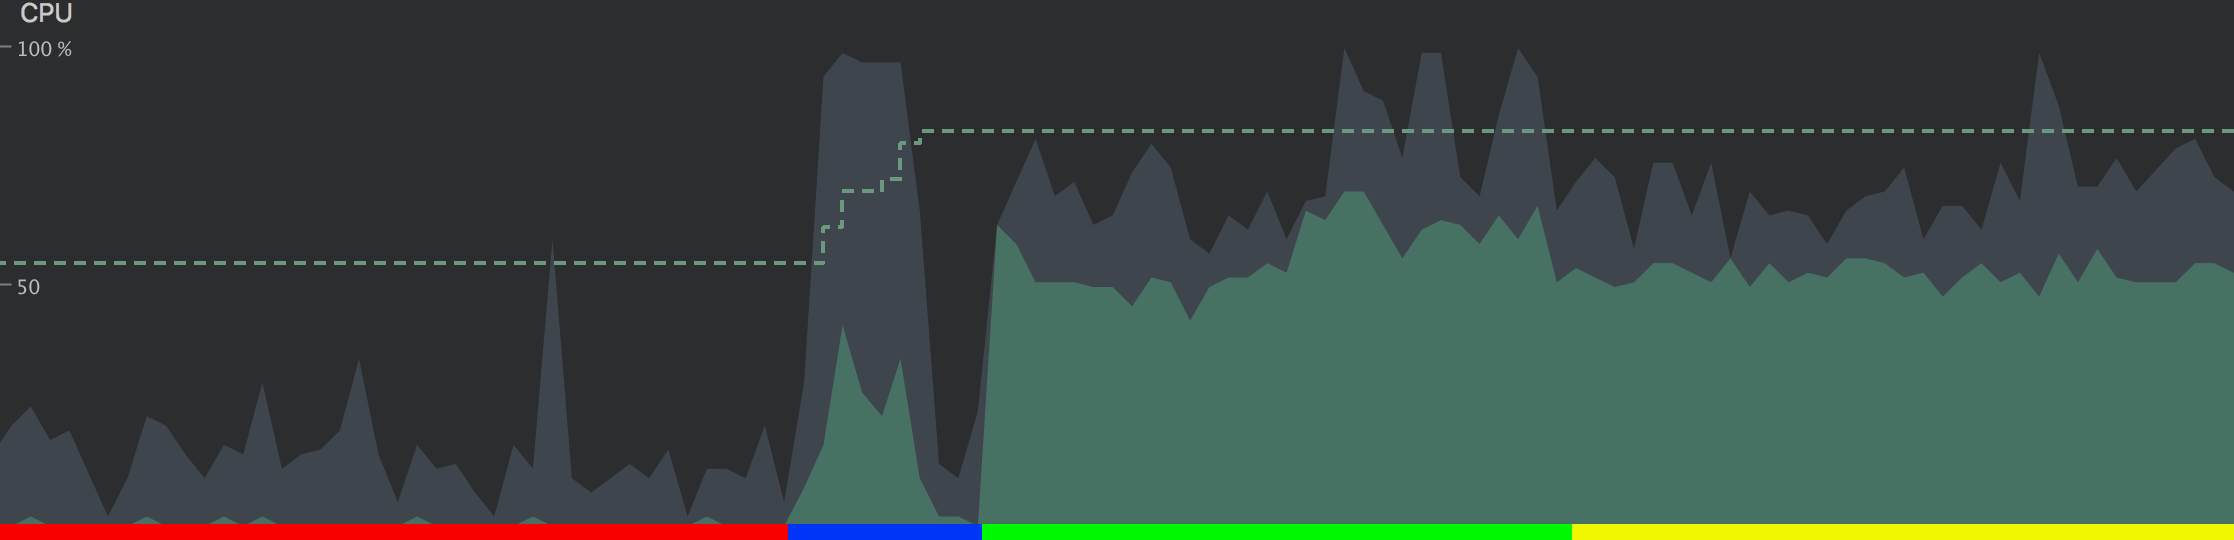
\includegraphics[height=3.5cm]{obrazky-figures/cpu_activity.png}
        \caption{Aktivita CPU při rozpoznávání, pořízeno pomocí Android Profiler}
\end{figure}

Z~tohoto obrázku je jasně vidět, že zdaleka výpočetně nejnáročnější částí celé implementace je dekódování. Výsledky testů doby výpočtu lze nalézt v~grafu \ref{graph:decoding_time}. Z~grafu je vidět, že zdvojnásobení velikosti slovníku vede přibližně k~dvojnásobně delší době výpočtu. Počet bigramů nemá na výpočetní dobu příliš velký vliv, při velikosti slovníku 1500 slov a počtu bigramů 77939 resp. 179832 je rozdíl v~době výpočtu pouze 0.2 s.

\begin{figure}[H]\label{graph:decoding_time}
\begin{center}
\begin{tikzpicture}
\begin{axis}[
	xlabel={velikost slovníku},
    y unit = s,
    ylabel={doba výpočtu}
]
\addplot table [x=size, y=time, mark=none, color=red]{data/compute_time.txt};
\end{axis}
\end{tikzpicture}
\end{center}
\caption{Vliv velikosti slovníku na dobu výpočtu}
\end{figure}

Z~grafu tedy vyplývá, že nejvhodnějším kandidátem pro rozpoznávání v~reálném čase je slovník o~velikosti 1500 slov.

Tabulka \ref{tab:memory_usage} zobrazuje využití paměti nativním kódem po načtení a alokování zdrojů pro různé slovníky. Z~tabulky je jasně vidět, že program vyžaduje velmi malé množství operační paměti pro svoje fungování.

\begin{table}[H]
\centering
\caption{Využití paměti při různých velikostech slovníku}
\label{tab:memory_usage}
\begin{tabular}{|l|l|l|}
\hline
Velikost slovníku & Počet bigramů & Využití paměti [MB] \\ \hline
20                & 0             & 8            \\ \hline
500               & 63706         & 11.2       \\ \hline
2000              & 81741         & 14        \\ \hline
5000              & 83128         & 19.4      \\ \hline
10000             & 83128         & 38.9        \\ \hline
\end{tabular}
\end{table}

\chapter{Závěr}
Cílem práce bylo implementovat jednotlivé části rozpoznávače řeči za použití nízkoúrovňových technologií platformy Android, cíl byl tedy splněn.

V~teoretické části dokumentu bylo popsáno, jak jsou zvuková data reprezentována ve výpočetních systémech a jakým způsobem se s~nimi pracuje. Je zde vysvětlen princip extrakce příznaků a vysvětluje jednotlivé kroky zmíněné extrakce. Dále popisuje princip dekódování za využití skrytých Markovových modelů a n-gramových jazykových modelů.

V~implementační části je uvedeno, jakým způsobem jsou data získána a dále zpracována. Blíže specifikuje, jak jsou data předávána v~rámci programu a vysvětluje, jakým způsobem jsou reprezentována. Také poukazuje na některé nedostatky implementace. Dále jsou v~dokumentu uvedena srovnání implementace extrakce příznaků v~různých jazycích, přičemž bylo zjištěno, že nejlepší možností je kombinace C++ a Renderscriptu.

Implementace extrakce příznaků, která byla realizována za použití NDK a Renderscriptu dodává stejné výsledky jako referenční implementace a doba jejich výpočtu je více než dostačující pro souběžné zpracování s~nahráváním zvukového signálu. Výpočetně nejnáročnější částí rozpoznávače je dekodér.

Kvůli vysoké výpočetní náročnosti dekódování audia je největším možným slovníkem pro rozpoznávání řeči v~reálném čase slovník o~velikosti přibližně $1500$ slov. Tato velikost slovníku není zdaleka vhodná pro diktování, proto by bylo vhodnější použít tuto implementaci spíše s~menším slovníkem, například pro řízení programu jednoduchými příkazy a přidaným post-processingem pro upřesnění rozpoznávání. Word error rate rozpoznávače se pohybuje na rozmezí $70-100\%$. Paměťová náročnost rozpoznávače je velmi malá a má velkou rezervu pro případné změny, které by využily větší množství paměťového prostoru.

Pravděpodobně nejlepším krokem dalšího vývoje by bylo přepracování dekodéru a prozkoumání možnosti využití Renderscriptu v~jeho implementaci. Dále by bylo vhodné přidat možnost získání nejen nejlepšího odhadu výsledku rozpoznávání, ale několika nejlepších. Důležitým dalším krokem je také samozřejmě zvýšení úspěšnosti rozpoznávače.
%=========================================================================
